%% This file is a portion of the source for Revised Edition 1.1 of
%% Operating Systems and Middleware: Supporting Controlled
%% Interaction, Copyright 2011 by Max Hailperin.  This work is
%% licensed under the Creative Commons Attribution-ShareAlike 3.0
%% Unported License. To view a copy of this license, visit
%% http://creativecommons.org/licenses/by-sa/3.0/ or send a letter to
%% Creative Commons, 171 Second Street, Suite 300, San Francisco,
%% California, 94105, USA.
\chapter{Synchronization and Deadlocks}
\label{synchronization-chapter}
\section{Introduction}

In Chapters \ref{threads-chapter} and \ref{scheduling-chapter}, you have seen how an operating system
can support concurrent threads of execution.  Now the time has come
to consider how the system supports controlled interaction
between those threads.  Because threads running at the same time on
the same computer can inherently interact by reading and writing a
common set of memory locations, the hard part is providing control.
In particular, this chapter will examine control over the
relative timing of execution steps that take place in differing
threads.

Recall that the scheduler is granted considerable authority to
temporarily preempt the execution of a thread and dispatch another
thread.  The scheduler may do so in response to unpredictable external
events, such as how long an I/O request takes to complete.  Therefore,
the computational steps taken by two (or more) threads will be
interleaved in a quite unpredictable manner, unless the programmer has
taken explicit measures to control the order of events.  Those control
measures are known as \vocab{synchronization}.
The usual way for synchronization to control event ordering is by causing
one thread to wait for another.

In Section~\ref{races-section}, I will provide a more detailed case for why
synchronization is needed by describing the problems that can occur
when interacting threads are not properly synchronized.  The
uncontrolled interactions are called races.  By examining some
typical races, I will illustrate the need for one particular form of
synchronization, mutual exclusion.  Mutual exclusion ensures that only
one
thread at a time can operate on a shared data structure or other
resource.  Section~\ref{mutexes-and-monitors-section} presents two
closely related ways mutual exclusion can be obtained. They are known as mutexes and monitors.

After covering mutual exclusion, I will turn to other, more general
synchronization challenges and to mechanisms that can address those
challenges.  To take one example, you may want to ensure that some
memory locations are read after they have been filled with useful
values, rather than before.  I devote Section~\ref{other-synchronization-problems-section} to enumerating
several of the most common synchronization patterns other than mutual
exclusion.  Afterward, I devote
Sections \ref{condition-variables-section} and \ref{semaphores-section} to two popular
mechanisms used to handle these situations. One, condition variables,
is an important extension to monitors; the combination of monitors
with condition variables allows many situations to be cleanly handled.
The other, semaphores, is an old favorite because it provides a
single, simple mechanism that in principle suffices for all
synchronization problems.  However, semaphores can be hard to
understand and use correctly.

Synchronization solves the problem of races, but it can create a new
problem of its own: deadlock.  Recall that synchronization typically
involves making threads wait; for example, in mutual exclusion, a
thread may need to wait its turn in order to enforce the rule of one
at a time.  Deadlock results when a cycle of waiting threads forms;
for example, thread A waits for thread B, which happens to be waiting
for thread A, as shown in Figure~\ref{scan-4-2}.
\begin{figure}
\centerline{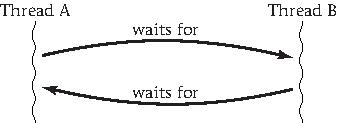
\includegraphics{hail_f0401}}
%\centerline{\epsfbox{scan-4-2.eps}}
\caption{Deadlock results when threads wait for one another in a
  complete cycle.  In this simple example, thread A is waiting for
  thread B, which is waiting for thread A.}
\label{scan-4-2}
\end{figure}
Because this pathology results from waiting, I
will address it and three of the most practical cures in Section~\ref{deadlock-section}, after
completing the study of waiting-based means of synchronization.

Waiting also interacts with scheduling (the topic of
Chapter~\ref{scheduling-chapter}) in some interesting ways.  In particular, unless special
precautions are taken, synchronization mechanisms can subvert priority
scheduling, allowing a low-priority thread to run while a
high-priority thread waits.  Therefore, in
Section~\ref{synchronization-and-scheduling-section}, I will briefly consider the
interactions between synchronization and scheduling, as well as what can be
done to tame them.

Although sections \ref{deadlock-section} and \ref{synchronization-and-scheduling-section} 
address the problems of deadlock and unwanted scheduling interactions, the root 
cause of these problems is also worth considering.
The underlying problem is that
one thread can block the progress of another thread, which is undesirable
even in the absence of such dramatic symptoms as deadlock.  After all, a blocked thread can't take
advantage of available processing power to produce useful results.  
Alternative, nonblocking synchronization techniques have become increasingly important
as the number of processor cores in a typical computer system has grown.
Section~\ref{nonblocking-synchronization-section} briefly addresses this topic, 
showing how data structures can safely support concurrent threads without ever blocking progress.

Finally, I conclude the chapter in
Section~\ref{synchronization-and-security-section} by looking at security issues related
to synchronization.  In particular, I show how subtle synchronization
bugs, which may nearly never cause a malfunction unless provoked, can
be exploited by an attacker in order to circumvent the system's normal
security policies.
After this concluding section, I provide exercises, programming and exploration projects, and notes.

Despite the wide range of synchronization-related topics I cover in
this chapter, there are two I leave for later chapters.
Atomic transactions are a particularly sophisticated and important
synchronization pattern, commonly encountered in middleware;
therefore, I devote Chapter~\ref{transactions-chapter} entirely to them.  Also,
explicitly passing a message between threads (for example, via a network)
provides synchronization as well as communication, because the message
cannot be received until after it has been transmitted.  Despite this
synchronization role, I chose to address various forms of message
passing in Chapters \ref{networking-chapter} and
\ref{distmid-chapter}, the chapters related to communication.

\section{Races and the Need for Mutual Exclusion}\label{races-section}

When two or more threads operate on a shared data structure, some very
strange malfunctions can occur if the timing of the threads turns out
precisely so that they
interfere with one another.  For example, consider the following
code that might appear in a \verb|sellTicket| procedure (for an event
without assigned seats):
\begin{verbatim}
if(seatsRemaining > 0){
  dispenseTicket();
  seatsRemaining = seatsRemaining - 1;
} else
  displaySorrySoldOut();
\end{verbatim}

On the surface, this code looks like it should never sell more tickets
than seats are available.  However, what happens if multiple threads
(perhaps controlling different points of sale) are executing the same
code?  Most of the time, all will be well.  Even if two people try to
buy tickets at what humans perceive as the same moment, on the time scale of
the computer, probably one will happen first and the other second, as
shown in Figure~\ref{ticket-ok-figure}.
\begin{figure}
\centerline{\begin{tabular}{|l|l|}
\hline\multicolumn{1}{|c|}{\bf Thread A} & \multicolumn{1}{c|}{\bf Thread B}\\\hline
\tt if(seatsRemaining > 0) & \\
\tt dispenseTicket(); & \\
\tt seatsRemaining=seatsRemaining-1; & \\
&\tt if(seatsRemaining > 0)...else \\
&\tt displaySorrySoldOut(); \\\hline
\end{tabular}}
\caption{Even if two humans think they are trying to buy the last
  ticket at the same time, chances are good that one's thread (thread A
  in this example) will run before the other's.  Thread B will then
  correctly discover that no seats remain.}\label{ticket-ok-figure}
\end{figure}
In that case, all is well.  However, once in a blue moon, the timing may be
exactly wrong, and the following scenario results, as shown in
Figure~\ref{ticket-race-figure}.
\begin{figure}
\centerline{\begin{tabular}{|l|l|}
\hline\multicolumn{1}{|c|}{\bf Thread A} & \multicolumn{1}{c|}{\bf Thread B}\\\hline
\tt if(seatsRemaining > 0) & \\
&\tt if(seatsRemaining > 0) \\
\tt dispenseTicket(); & \\
&\tt dispenseTicket(); \\
\tt seatsRemaining=seatsRemaining-1; & \\
&\tt seatsRemaining=seatsRemaining-1;  \\\hline
\end{tabular}}
\caption{If threads A and B are interleaved, both can act as though
  there were a ticket left to sell, even though only one really exists
  for the two of them.}\label{ticket-race-figure}
\end{figure}
\begin{enumerate}
\item
Thread A checks \verb|seatsRemaining > 0|.  Because
\verb|seatsRemaining| is 1, the test succeeds.  Thread A will take the
first branch of the \verb|if|.
\item
Thread B checks \verb|seatsRemaining > 0|.  Because
\verb|seatsRemaining| is 1, the test succeeds.  Thread B will take the
first branch of the \verb|if|.
\item
Thread A dispenses a ticket and decreases \verb|seatsRemaining| to 0.
\item
Thread B dispenses a ticket and decreases \verb|seatsRemaining| to $-1$.
\item
One customer winds up sitting on the lap of another.
\end{enumerate}

Of course, there are plenty of other equally unlikely scenarios that
result in misbehavior.  In Exercise~\ref{race-exercise}, you can come
up with a scenario
where, starting with \verb|seatsRemaining| being 2, two threads each
dispense a ticket, but \verb|seatsRemaining| is left as 1 rather than
0.

These scenarios are examples of \vocabs{race}.  In a race, 
two threads use the same data structure, without any mechanism to
ensure only one thread uses the data structure at a time.  If either thread precedes the
other, all is well.  However, if the two are interleaved, the program
malfunctions.  Generally, the malfunction can be expressed as some
invariant property being violated.  In the ticket-sales example, the
invariant is that the value of \verb|seatsRemaining|
should be nonnegative and when added to
the number
of tickets dispensed should equal the total number of seats.
(This invariant assumes that \verb|seatsRemaining| was initialized to
the total number of seats.)

When an invariant involves more than one variable, a race can result
even if one of the threads only reads the variables, without modifying
them.  For example, suppose there are two variables, one recording how
many tickets have been sold and the other recording the amount of
cash in the money drawer.  There should be an invariant relation between
these: the number of tickets sold times the price per ticket, plus the
amount of starting cash, should equal the cash on hand.  Suppose one
thread is in the midst of selling a ticket.  It has updated one of the
variables, but not yet the other.  If at exactly that moment another
thread chooses to run an audit function, which inspects the values of
the two variables, it will find them in an inconsistent state.

That inconsistency may not sound so terrible, but what if a similar
inconsistency occurred in a
medical setting, and one variable recorded the drug to administer,
while the other recorded the dose?  Can you see how dangerous an
inconsistency could be?  Something very much like that happened in a
radiation therapy machine, the \index{Therac-25}Therac-25, with occasionally lethal
consequences.  (Worse, some patients suffered terrible but not
immediately lethal injuries and lingered for some time in
excruciating, intractable pain.)

From the ticket-sales example, you can see that having two
threads carrying out operations on the same data structure is
harmless, as long as there never are two operations under way at the
same time.  In other words, the interleaving of the threads' execution
needs to be at the granularity of complete operations, such as selling
a ticket or auditing the cash drawer.  When interleaving the operations,
it's OK if one thread performs
several complete operations in a row; the threads don't need to alternate back and forth.
However, each sale or audit should be completed without interruption.

The reason why any interleaving of complete operations is safe is
because each is designed to both rely on the invariant and preserve
it.  Provided that you initially construct the data structure in a state
where the invariant holds, any sequence whatsoever of
invariant-preserving operations will leave the invariant intact.

What is needed, then, is a synchronization mechanism that allows one
thread to obtain private access to the data structure before it begins work, thereby
excluding all other threads from operating on that structure.  The
conventional metaphor is to say that the thread \vocabs{lock} the data structure.
When
the thread that locked the structure is done, it unlocks, allowing
another thread to take its turn.  Because any thread in the midst of
one of the operations temporarily excludes all the others,
this arrangement is called \foldvocab{mutual}{exclusion}.  Mutual exclusion establishes the
granularity at which threads may be interleaved by the scheduler.

\section{Mutexes and Monitors}\label{mutexes-and-monitors-section}

As you saw in Section~\ref{races-section}, threads that share data structures
need to have a mechanism for obtaining exclusive access to those
structures.  A programmer can arrange for this exclusive access by
creating a special lock object associated with each shared data
structure.  The lock can only be locked by one thread at a time.
A thread that has locked the lock is said to \vocabindex{hold}{hold (a lock)} the lock, even though that vocabulary has no obvious connection to the metaphor of real-world locks.
If
the threads operate on (or even examine) the data structure
only when holding the corresponding lock, this discipline will prevent
races.

To
support this form of race prevention, operating systems and middleware generally
provide mutual exclusion locks.  Because the name \foldvocab{mutual exclusion}{lock}
is rather ungainly, something shorter is generally used.  Some
programmers simply talk of \vocabs{lock}, but that can lead to confusion
because other synchronization mechanisms are also called locks. (For
example, I introduce readers/writers locks in Section~\ref{rw-section}.)  Therefore, the
name \vocab{mutex} has become popular as a shortened form of \foldvocab{mutual
exclusion}{lock}.  In particular, the POSIX standard refers to
mutexes.  Therefore, I will use that name in this book as well.

Section~\ref{mutex-api-section} presents the POSIX application
programming interface (API) for
mutexes. Section~\ref{monitors-section} presents an alternative, more
structured interface to mutexes, known as monitors.  Finally,
Section~\ref{mutex-mechanisms-section} shows what lies behind both
of those interfaces by explaining the mechanisms typically used to
implement mutexes.

\subsection{The Mutex Application Programing Interface}\label{mutex-api-section}

A mutex can be in either of two states: locked (that is, held by some
thread), or unlocked (that is, not held by any thread).  Any
implementation of mutexes must have some way to create a mutex and
initialize its state.  Conventionally, mutexes are initialized to the
unlocked state.  As a minimum, there must be two other operations: one
to lock a mutex, and one to unlock it.

The lock and unlock operations are much less symmetrical than they
sound.  The unlock operation can be applied only when the mutex is
locked; this operation does its job
and returns, without making the calling thread wait.  The lock
operation, on the other hand, can be invoked even when the lock is
already locked.  For this reason, the calling thread may need to wait, as shown in
Figure~\ref{scan-4-3}.
\begin{figure}
\centerline{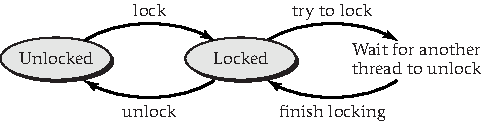
\includegraphics{hail_f0404}}
%\centerline{\epsfbox{scan-4-3.eps}}
\caption{Locking an unlocked mutex and unlocking a locked one change
  the mutex's state.  However, a thread can also try to lock an
  already-locked mutex.  In this case, the thread waits and acquires
  the mutex lock when another thread unlocks it.}
\label{scan-4-3}
\end{figure}
When a thread invokes the lock operation on a mutex, and that mutex is
already in the locked state, the thread is made to wait until another
thread has unlocked the mutex.  At that point, the thread that wanted
to lock the mutex can resume execution, find the mutex unlocked, lock
it, and proceed.

If more than one thread is trying to lock the same
mutex, only one of them will switch the mutex from unlocked to locked;
that thread will be allowed to proceed.  The others will wait until
the mutex is again unlocked.  This behavior of the lock operation
provides mutual exclusion.  For a thread to proceed past the point
where it invokes the lock operation, it must be the single thread that
succeeds in switching the mutex from unlocked to locked.  Until the
thread unlocks the mutex, one can say it \vocabindex{holds}{hold (a lock)} the mutex (that is, has
exclusive rights) and can safely operate on the associated data
structure in a race-free fashion.

This freedom from races exists regardless which one of the waiting
threads is chosen as the one to lock the mutex.  However, the question of
which thread goes first may matter for other reasons; I return to it
in Section~\ref{convoy-section}.

Besides the basic operations to initialize a mutex, lock it, and
unlock it, there may be other, less essential, operations as well.
For example, there may be one to test whether a mutex is immediately
lockable without waiting, and then to lock it if it is so.  For systems that
rely on manual reclamation of memory, there may also be an operation
to destroy a mutex when it will no longer be used.

Individual operating systems and middleware systems provide mutex APIs
that fit the general pattern I described, with varying details.
In order to see one concrete example of an API, I will present the
mutex operations included in the POSIX standard.  Because this is a
standard, many different operating systems provide this API, as well
as perhaps other system-specific APIs.

In the POSIX API, you can declare \verb|my_mutex| to be a mutex and
initialize it with the default attributes as follows:
\index{pthread_mutex_t@\verb"|pthread_mutex_t"|}%
\index{pthread_mutex_init@\verb"|pthread_mutex_init"|}%
\begin{verbatim}
pthread_mutex_t my_mutex;
pthread_mutex_init(&my_mutex, 0);
\end{verbatim}
A thread that wants to lock the mutex, operate on the associated data
structure, and then unlock the mutex would do the following (perhaps
with some error-checking added):
\index{pthread_mutex_lock@\verb"|pthread_mutex_lock"|}%
\index{pthread_mutex_unlock@\verb"|pthread_mutex_unlock"|}%
\begin{verbatim}
pthread_mutex_lock(&my_mutex);
// operate on the protected data structure
pthread_mutex_unlock(&my_mutex);
\end{verbatim}
As an example, Figure~\ref{tickets-pthreads-code} shows the key
procedures from the ticket sales example, written in C using the POSIX API.
\begin{figure}
\begin{verbatim}
void sellTicket(){
  pthread_mutex_lock(&my_mutex);
  if(seatsRemaining > 0){
    dispenseTicket();
    seatsRemaining = seatsRemaining - 1;
    cashOnHand = cashOnHand + PRICE;
  } else
    displaySorrySoldOut();
  pthread_mutex_unlock(&my_mutex);
}

void audit(){
  pthread_mutex_lock(&my_mutex);
  int revenue = (TOTAL_SEATS - seatsRemaining) * PRICE;
  if(cashOnHand != revenue + STARTING_CASH){
    printf("Cash fails to match.\n");
    exit(1);
  }
  pthread_mutex_unlock(&my_mutex);
}
\end{verbatim}
\caption{Each of these procedures begins by locking {\tt my\_mutex} and
  ends by unlocking it.  Therefore, they will never race, even if
  called from concurrent threads. Additional code not shown here
  (perhaps in the main procedure) would first initialize {\tt my\_mutex}.}
\label{tickets-pthreads-code}
\end{figure}
When all threads are done using the mutex (leaving it in the unlocked
state), the programmer is expected to destroy it, so that any
underlying memory can be reclaimed.  This is done by
executing the following procedure call:
\index{pthread_mutex_destroy@\verb"|pthread_mutex_destroy"|}%
\begin{verbatim}
pthread_mutex_destroy(&my_mutex);
\end{verbatim}

POSIX also provides a couple variants on \verb|pthread_mutex_lock|
that are useful under particular circumstances.  One,
\index{pthread_mutex_trylock@\verb"|pthread_mutex_trylock"|}\verb|pthread_mutex_trylock|, differs in that it will never wait to
acquire a mutex. Instead, it returns an error code if unable to
immediately acquire the lock.  The other,
\index{pthread_mutex_timedlock@\verb"|pthread_mutex_timedlock"|}\verb|pthread_mutex_timedlock|, allows the programmer to specify a
maximum amount of time to wait.  If the mutex cannot be acquired
within that time, \verb|pthread_mutex_timedlock| returns an error
code.

Beyond their wide availability, another reason why POSIX mutexes are
worth studying is that the programmer is allowed to choose among several
variants, which provide different answers to two questions about exceptional
circumstances.
Other mutex APIs might include one specific answer to these questions,
rather than exposing the full range of possibilities.  The questions
at issue are as follows:
\begin{itemize}
\item
What happens if a thread tries to unlock a mutex that is unlocked, or that was locked by a
different thread?
\item
What happens if a thread tries to lock a mutex that it already holds?
(Note that if the thread were to wait for itself to unlock the mutex,
this situation would constitute the simplest possible case of a deadlock.  The cycle of
waiting threads would consist of a single thread, waiting for itself.)
\end{itemize}

The POSIX standard allows the programmer to select from four different
types of mutexes, each of which answers these two questions in a
different way:
\begin{description}
\item[\texttt{PTHREAD\_MUTEX\_DEFAULT}]
If a thread tries to
lock a mutex it already holds or unlock one it doesn't hold, all bets are off as to what will happen.
The programmer has a responsibility never to make either of these attempts.
Different POSIX-compliant systems may behave differently.
\item[\texttt{PTHREAD\_MUTEX\_ERROR\_CHECK}]
If a thread tries to lock a mutex that it already holds, or unlock a
mutex that it doesn't hold, the operation returns an error code.
\item[\texttt{PTHREAD\_MUTEX\_NORMAL}]
If a thread tries to lock a mutex that it already holds, it goes into
a deadlock situation, waiting for itself to unlock the mutex, just
as it would wait for any other thread.  If a thread tries to unlock
a mutex that it doesn't hold, all bets are off; each POSIX-compliant
system is free to respond however it likes.
\item[\texttt{PTHREAD\_MUTEX\_RECURSIVE}]
If a thread tries to unlock a mutex that it doesn't hold, the
operation returns an error code.  If a thread tries to lock a mutex
that it already holds, the system simply increments a count of how
many times the thread has locked the mutex and allows the thread to
proceed.  When the thread invokes the unlock operation, the counter is
decremented, and only when it reaches 0 is the mutex really unlocked.
\end{description}

If you want to provoke a debate among experts on concurrent
programming, ask their opinion of \vocab{recursive locking}, that is,
of the mutex behavior specified by the POSIX option \texttt{PTHREAD\_MUTEX\_RECURSIVE}.
On the one hand, recursive locking gets rid of one especially silly
class of deadlocks, in which a thread waits for a mutex it already holds.
On the other hand, a programmer with recursive locking available may
not follow as disciplined a development approach. In particular, the programmer
may not keep track of exactly which locks are held at each point
in the program's execution.

\subsection{Monitors: A More Structured Interface to Mutexes}\label{monitors-section}

Object-oriented programming involves packaging together data
structures with the procedures that operate on them.  In this context,
mutexes can be used in a very rigidly structured way:
\begin{itemize}
\item
All state variables within an object should be kept private, accessible only to
code associated with that object.
\item
Every object (that might be shared between threads) should contain a
mutex as an additional field, beyond those fields containing the object's
state.
\item
Every method of an object (except private ones used internally) should
start by locking that object's mutex and end by unlocking the mutex
immediately before returning.
\end{itemize}
If these three rules are followed, then it will be impossible for two
threads to race on the state of an object, because all access to the
object's state will be protected by the object's mutex.

Programmers can follow these rules manually, or the programming
language can provide automatic support for the rules.  Automation
ensures that the rules are consistently followed.  It also means the
source program will not be cluttered with mutex clich{\'e}s, and hence
will be more readable.

An object that automatically follows the mutex rules is called a
\vocab{monitor}.  Monitors are found in some programming languages,
such as Concurrent Pascal, that
have been used in research settings without becoming commercially
popular.  In these languages, using monitors can be as simple as using
the keyword \verb|monitor| at the
beginning of a declaration for a class of objects.  All public methods
will then automatically lock and unlock an automatically supplied
mutex.  (Monitor languages also support another synchronization
feature, condition variables, which I discuss in Section~\ref{condition-variables-section}.)


Although true monitors have not become popular, the Java programming
language provides a close approximation.  To achieve monitor-style
synchronization, the Java programmer needs to exercise some self-discipline, but less than with raw mutexes.  More importantly, the
resulting Java program is essentially as uncluttered as a true monitor
program would be; all that is added is one keyword,
\verb|synchronized|, at the declaration of each nonprivate method.

Each Java object automatically has a mutex associated with it, of the
recursively lockable kind.  The programmer can choose to lock any
object's mutex for the duration of any block of code by using a
\index{synchronized statement@\verb"|synchronized"| statement}\verb|synchronized| statement:
\begin{verbatim}
synchronized(someObject){
  // the code to do while holding someObject's mutex
}
\end{verbatim}
Note that in this case, the code need not be operating on the state of
\verb|someObject|; nor does this code need to be in a method
associated with that object.  In other words, the \verb|synchronized|
statement is essentially as flexible as using raw mutexes, with the
one key advantage that locking and unlocking are automatically paired.
This advantage is important, because it eliminates one big class of
programming errors.  Programmers often forget to unlock mutexes under
exceptional circumstances.  For example, a procedure may lock a mutex
at the beginning and unlock it at the end.  However, in between may
come an \verb|if| statement that can terminate the procedure with
the mutex still locked.

Although the \verb|synchronized|
statement is flexible, typical Java programs don't use it much.  Instead, programmers add the keyword
\index{synchronized method@\verb"|synchronized"| method}\verb|synchronized| to the declaration of public methods.  For
example, a \verb|TicketVendor| class might follow the outline in
Figure~\ref{TicketVendor}.
\begin{figure}
\begin{verbatim}
public class TicketVendor {
  private int seatsRemaining, cashOnHand;
  private static final int PRICE = 1000;

  public synchronized void sellTicket(){
    if(seatsRemaining > 0){
      dispenseTicket();
      seatsRemaining = seatsRemaining - 1;
      cashOnHand = cashOnHand + PRICE;
    } else
      displaySorrySoldOut();
  }

  public synchronized void audit(){
    // check seatsRemaining, cashOnHand
  }

  private void dispenseTicket(){
    // ...
  }

  private void displaySorrySoldOut(){
    // ...
  }

  public TicketVendor(){
    // ...
  }
}
\end{verbatim}
\caption{Outline of a monitor-style class in Java}
\label{TicketVendor}
\end{figure}
Marking a method \verb|synchronized| is
equivalent to wrapping the entire body of that method in
a \verb|synchronized| statement:
\begin{verbatim}
synchronized(this){
  // the body
}
\end{verbatim}
In other words, a synchronized method on an object will be executed
while holding that object's mutex.  For example, the \verb|sellTicket|
method is synchronized, so if two different threads invoke it, one
will be served while the other waits its turn, because the
\verb|sellTicket| method is implicitly locking a mutex upon entry and
unlocking it upon return, just as was done explicitly in the POSIX
version of Figure~\ref{tickets-pthreads-code}.  Similarly, a thread
executing the \verb|audit| method will need to wait until no ticket
sale is in progress, because this method is also marked synchronized,
and so acquires the same mutex.

In order to program in a monitor style in Java, you need to be
disciplined in your use of the \verb|private| and \verb|public|
keywords (including making all state \verb|private|), and you need to
mark all the public methods as \verb|synchronized|.

\subsection{Underlying Mechanisms for Mutexes}\label{mutex-mechanisms-section}

In this subsection, I will show how mutexes typically operate behind
the scenes.  I start with a version that functions correctly, but is
inefficient, and then show how to build a more efficient version on
top of it, and then a yet more efficient version on top of that.  Keep
in mind that I will not throw away my first two versions: they play
a critical role in the final version.  For simplicity, all three
versions will be of the \texttt{PTHREAD\_MUTEX\_NORMAL} kind;
a deadlock results if a thread tries to lock a mutex it already
holds.  In Exercise~\ref{recursive-mutex-exercise},
you can figure out the changes needed for \texttt{PTHREAD\_MUTEX\_RECURSIVE}.

The three versions of mutex are called the basic spinlock,
cache-conscious spinlock, and queuing mutex, in increasing order of
sophistication.  The meaning of these names will become apparent as I
explain the functioning of each kind of mutex.  I will start with the
basic spinlock.

All modern processor architectures have at least one instruction that
can be used to both change the contents of a memory location and
obtain information about the previous contents of the location.
Crucially, these instructions are executed \vocabindex{atomically}{atomic}, that is, as
an indivisible unit that cannot be broken up by the arrival of an
interrupt nor interleaved with the execution of an instruction on
another processor.  The details of these instructions vary; for
concreteness, I will use the \vocab{exchange} operation, which atomically
swaps the contents of a register with the contents of a memory
location.

Suppose I represent a basic spinlock as a memory location that contains 1 if
the mutex is unlocked and 0 if the mutex is locked.  The unlock
operation can be trivial: to unlock a mutex, just store 1 into it.
The lock operation is a bit trickier and uses the atomic exchange
operation; I can express it in pseudocode, as shown in
Figure~\ref{basic-spinlock-lock}.
\begin{figure}
\begin{verbatim}
to lock mutex:
  let temp = 0
  repeat
    atomically exchange temp and mutex
  until temp = 1
\end{verbatim}
\caption{The basic spinlock version of a mutex is a memory location
  storing 1 for unlocked and 0 for locked.  Locking the mutex consists of
  repeatedly exchanging a register containing 0 with the memory
  location until the location is changed from 1 to 0.}
\label{basic-spinlock-lock}
\end{figure}
The key idea here is to keep looping until the thread succeeds in changing the
mutex from 1 to 0.  So long as some other thread holds the
lock, the thread keeps swapping one 0 with another 0, which does no harm.
This process is illustrated in Figure~\ref{scan-4-4}.
\begin{figure}
\centerline{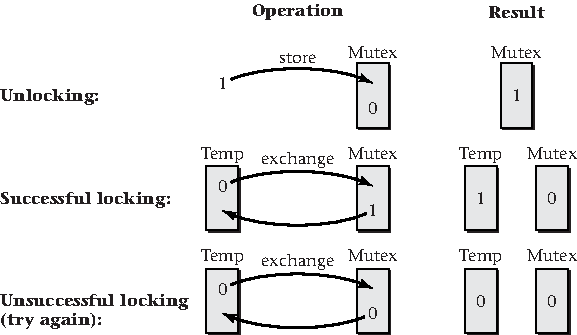
\includegraphics{hail_f0408}}
%\centerline{\epsfbox{scan-4-4.eps}}
\caption{Unlocking a basic spinlock consists of storing a 1 into it.
  Locking it consists of storing a 0 into it using an atomic exchange
  instruction.  The exchange instruction allows the locking thread to verify that the
  value in memory really was changed from 1 to 0.  If not, the thread
  repeats the attempt.}
\label{scan-4-4}
\end{figure}

To understand the motivation behind the cache-conscious spinlock, you need to
know a little about \foldindex{cache}{coherence}cache coherence
protocols in \index{multiprocessor system}multiprocessor
systems.  Copies of a given block of memory can reside in several
different processors' caches, as long as the processors only read from the
memory locations.  As soon as one processor wants to write into the
cache block, however, some communication between the caches is
necessary so that other processors don't read out-of-date
values.  Most typically, the cache where the writing occurs invalidates all the other caches' copies so
that it has exclusive ownership.  If one of the other processors now
wants to write, the block needs to be flushed out of the first cache
and loaded exclusively into the second.  If the two processors keep
alternately writing into the same block, there will be continual
traffic on the memory interconnect as the cache block is transferred
back and forth between the two caches.

This is exactly what will happen with the basic spinlock version of mutex
locking if two threads (on two processors) are both waiting for the
same lock.  The atomic exchange instructions on the two processors will
both be writing into the cache block containing the spinlock.
Contention for a mutex may not
happen often.  When it does, however, the performance will be
sufficiently terrible to motivate an improvement. Cache-conscious spinlocks
will use the same simple approach as basic spinlocks  when there is no
contention, but will get rid of the cache coherence traffic while waiting
for a contended mutex.

In order to allow multiple processors to wait for a lock without
generating traffic outside their individual caches, they must be
waiting while using only reads of the mutex.  When they see the mutex become
unlocked, they then need to try grabbing it with an atomic
exchange.  This approach leads to the pseudocode shown in Figure~\ref{cache-conscious-lock}.
\begin{figure}
\begin{verbatim}
to lock mutex:
  let temp = 0
  repeat
    atomically exchange temp and mutex
    if temp = 0 then
      while mutex = 0
        do nothing
  until temp = 1
\end{verbatim}
\caption{Cache-conscious spinlocks are represented the same way as
  basic spinlocks, using a single memory location.  However, the lock
  operation now uses ordinary read instructions in place of most of
  the atomic exchanges while waiting for the mutex to be unlocked.}
\label{cache-conscious-lock}
\end{figure}
Notice that in the common case where the mutex can be acquired
immediately, this version acts just like the original.  Only if the
attempt to acquire the mutex fails is anything done differently.  Even
then, the mutex will eventually be acquired the same way as before.

The two versions of mutexes that I have presented thus far share one
key property, which explains why both are called spinlocks.
They both engage in \foldindex{busy}{waiting}busy waiting if the mutex
is not immediately available.  Recall from my discussion of scheduling
that busy waiting means waiting by continually executing instructions
that check for the awaited event.  A mutex that uses busy waiting is
called a \vocab{spinlock}.  Even fancier versions of spinlocks exist,
as described in the end-of-chapter notes.

The alternative to busy waiting is to notify the operating system that
the thread needs to wait.  The operating system can then change the
thread's state to waiting and move it to a
wait queue, where it is not eligible for time on the processor.
Instead, the scheduler will use the processor to run other threads.
When the mutex is unlocked, the waiting thread can be made runnable
again.  Because this form of mutex makes use of a wait queue, it is
called a queuing mutex.

Spinlocks are inefficient, for the same reason as any busy waiting is inefficient.
The thread does not make any more headway, no matter how many times it
spins around its loop.  Therefore, using the processor for a different
thread would benefit that other thread without harming the waiting
one.

However, there is one flaw in this argument.  There is some overhead
cost for notifying the operating system of the desire to wait,
changing the thread's state, and doing a context switch, with the
attendant loss of cache locality.  Thus, in a situation where the
spinlock needs to spin only briefly before finding the mutex unlocked,
the thread might actually waste less time busy waiting than it would waste
getting out of other threads' ways.  The relative efficiency of
spinlocks and queuing mutexes
depends on how long the thread needs to wait before the
mutex becomes available.

For this reason, spinlocks are appropriate to use for mutexes that are
held only very briefly, and hence should be quickly acquirable.
As an example, the Linux kernel uses spinlocks to protect many of its
internal data structures during the brief operations on them.  For
example, I mentioned that the scheduler keeps the runnable threads in
a run queue.  Whenever the scheduler wants to
insert a thread into this data structure, or otherwise operate on
it, it locks a spinlock, does the brief operation, and then
unlocks the spinlock.

Queuing mutexes are still needed for those cases where a
thread might hold a mutex a long time---long enough that other
contenders shouldn't busy wait.  These mutexes will be more complex.
Rather than being stored in a single memory location (as with
spinlocks), each mutex will have three components:
\begin{itemize}
\item
A memory location used to record the mutex's state, 1 for unlocked or
0 for locked.
\item
A list of threads waiting to acquire the mutex.  This list is what
allows the scheduler to place the threads in a waiting state, instead
of busy waiting.  Using the terminology of
Chapter~\ref{scheduling-chapter}, this list is a wait queue.
\item
A cache-conscious spinlock, used to protect against races in
operations on the mutex itself.
\end{itemize}
In my pseudocode, I will refer to these three components as
\verb|mutex.state|, \verb|mutex.waiters|, and \verb|mutex.spinlock|,
respectively.

Under these assumptions, the locking and unlocking operations can be
performed as shown in the pseudocode of Figures \ref{lock-pseudo-code} and
\ref{unlock-pseudo-code}.  Figures \ref{scan-4-5} and \ref{scan-4-6}
illustrate the functioning of these operations.
\begin{figure}
\begin{verbatim}
to lock mutex:
  lock mutex.spinlock (in cache-conscious fashion)
  if mutex.state = 1 then
    let mutex.state = 0
    unlock mutex.spinlock
  else
    add current thread to mutex.waiters
    remove current thread from runnable threads
    unlock mutex.spinlock
    yield to a runnable thread
\end{verbatim}
\caption{An attempt to lock a queuing mutex that is already in the
  locked state causes the thread to join the wait queue, {\tt mutex.waiters}.}
\label{lock-pseudo-code}
\end{figure}
\begin{figure}
\begin{verbatim}
to unlock mutex:
  lock mutex.spinlock (in cache-conscious fashion)
  if mutex.waiters is empty then
    let mutex.state = 1
  else
    move one thread from mutex.waiters to runnable
  unlock mutex.spinlock
\end{verbatim}
\caption{If there is any waiting thread, the unlock operation on a queuing mutex causes a thread to become
  runnable. Note that in this case, the mutex is left in the locked
  state; effectively, the locked mutex is being passed directly from
  one thread to another.}
\label{unlock-pseudo-code}
\end{figure}
\begin{figure}
\centerline{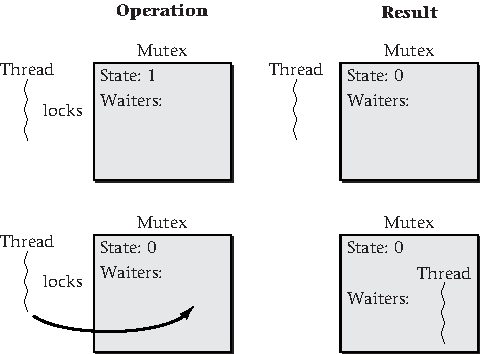
\includegraphics{hail_f0412}}
%\centerline{\epsfbox{scan-4-5.eps}}
\caption{Locking a queuing mutex that is unlocked simply changes the
  mutex's state.  Locking an already-locked queuing mutex, on the
  other hand, puts the thread into the waiters list.}
\label{scan-4-5}
\end{figure}
\begin{figure}
\centerline{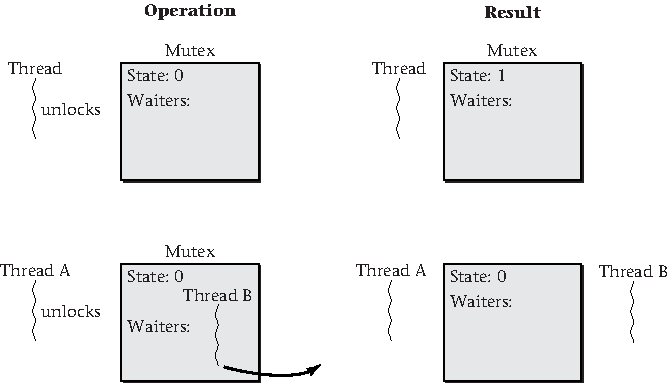
\includegraphics{hail_f0413}}
%\centerline{\epsfbox{scan-4-6.eps}}
\caption{Unlocking a queuing mutex with no waiting threads simply
  changes the mutex's state.  Unlocking a queuing mutex with waiting
  threads, on the other hand, leaves the state set to locked but
  causes one of the waiting threads to start running again, having
  acquired the lock.}
\label{scan-4-6}
\end{figure}
One important feature to note in this mutex design concerns what
happens when a thread performs the unlock operation on a mutex that has one or more threads in the
waiters list.  As you can see in Figure~\ref{unlock-pseudo-code}, the
mutex's state variable is not changed from the locked state (0) to the
unlocked state (1).  Instead, the mutex is left locked, and one of the
waiting threads is woken up.  In other words, the locked mutex is
passed directly from one thread to another, without ever really being
unlocked.  In Section~\ref{convoy-section}, I will explain how this
design is partially responsible for the so-called convoy
phenomenon, which I describe there.  In that same section, I will also present an
alternative design for mutexes that puts the mutex into the unlocked
state.

\section{Other Synchronization Patterns}\label{other-synchronization-problems-section}

Recall that synchronization refers to any form of control over the
relative timing of two or more threads.  As such, synchronization
includes more than just mutual exclusion; a programmer may want to impose some
restriction on relative timing other than the rule of one thread at a
time.  In this section, I present three other patterns of
synchronization that crop up over and over again in many applications:
bounded buffers, readers/writers locks, and barriers.
Sections \ref{bounded-buffers-section} through 
\ref{barriers-section} will just describe the desired synchronization;
Sections \ref{condition-variables-section} and \ref{semaphores-section} show techniques that can be used to achieve the
synchronization.

\subsection{Bounded Buffers}\label{bounded-buffers-section}

Often, two threads are linked together in a processing
\vocab{pipeline}.  That is,
the first thread produces a sequence of values that are consumed by
the second thread.  For example, the first thread may be extracting
all the textual words from a document (by skipping over the formatting
codes) and passing those words to a second thread that speaks the
words aloud.

One simple way to organize the processing would be by strict
alternation between the producing and consuming threads.  In the preceding
example, the first thread would extract a word, and then wait while
the second thread converted it into sound.  The second thread would
then wait while the first thread extracted the next word.  However,
this approach doesn't yield any concurrency: only one thread is
runnable at a time.  This lack of concurrency may result in suboptimal
performance if the computer system has two processors, or
if one of the threads spends a lot of time waiting for an I/O device.

Instead, consider running the \index{producer}producer and the \index{consumer}consumer
concurrently.  Every time the producer has a new value ready, the producer will
store the value into an intermediate storage area, called a \vocab{buffer}.
Every time the consumer is ready for the next value, it will retrieve
the value from the buffer.  Under normal circumstances, each can operate at
its own pace.  However, if the consumer goes to the buffer to retrieve
a value and finds the buffer empty, the consumer will need to wait for the
producer to catch up.  Also, if you want to limit the size of the
buffer (that is, to use a \foldvocab{bounded}{buffer}), you need to make the producer wait
if it gets too far ahead of the consumer and fills the buffer.  Putting
these two synchronization restrictions in place ensures that over the
long haul, the rate of the two threads will match up, although
over the short term, either may run faster than the other.

You should be familiar with the bounded buffer pattern from businesses
in the real world.  For example, the cooks at a fast-food
restaurant fry burgers concurrently with the cashiers selling them.
In between the two is a bounded buffer of already-cooked burgers.
The exact number of burgers in the buffer will grow or shrink somewhat
as one group of workers is temporarily a little faster than the
other.  Only under extreme circumstances does one group of workers
have to wait for the other.  Figure~\ref{scan-4-7} illustrates a situation where no one needs to wait.
\begin{figure}
\centerline{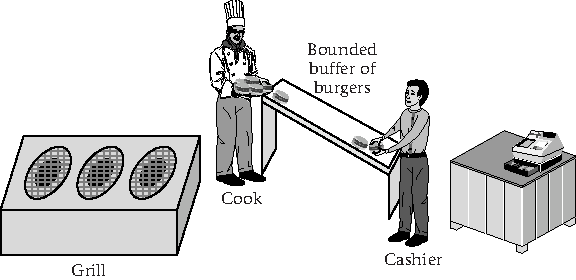
\includegraphics{hail_f0414}}
%\centerline{\epsfbox{scan-4-7.eps}}
\caption{A cook fries burgers and places them in a bounded buffer,
  queued up for later sale.  A cashier takes burgers from the
  buffer to sell.  If there are none available, the cashier waits.
  Similarly, if the buffer area is full, the cook takes a break from
  frying burgers.}
\label{scan-4-7}
\end{figure}


One easy place to see bounded buffers at work in computer systems is
the \vocab{pipe} feature built into UNIX-family operating systems,
including Linux and Mac OS~X.  (Microsoft Windows also now has an
analogous feature.)  Pipes allow the output produced by one process to
serve as input for another.  For example, on a Mac OS~X
system, you could open a terminal window with a shell in it and give the following command:
\begin{verbatim}
ls | say
\end{verbatim}
This runs two programs concurrently.  The first, \verb|ls|,
lists
the files in your current directory. 
The second one, \verb|say|, converts its textual input into speech and
plays it over the computer's speakers.   In the shell
command, the vertical bar character (\verb:|:) indicates the pipe from
the first program to the second. The net result is a spoken
listing of your files.

A more mundane version of this
example works not only on Mac OS~X, but also on other UNIX-family
systems such as Linux:
\begin{verbatim}
ls | tr a-z A-Z
\end{verbatim}
Again, this runs two programs concurrently.  This time the second one, \verb|tr|, copies
characters from its input to its output, with some changes
(transliterations) along the way; in this case, replacing lowercase
letters \verb|a-z| with the corresponding uppercase letters \verb|A-Z|.  The net
result is an uppercase listing of your files.  The file listing may
get ahead of the transliteration, as long as it doesn't overflow a
buffer the operating system provides for the pipe.  Once there is a
backlog of listed files in the buffer, the transliteration can run as
fast as it wants until it exhausts that backlog.

\subsection{Readers/Writers Locks}\label{rw-section}

My next example of a synchronization pattern is actually quite
similar to mutual exclusion.  Recall that in the ticket-sales
example, the audit function needed to acquire the mutex, even though auditing
is a read-only operation, in order to make sure that the audit read a consistent
combination of state variables.  That design achieved correctness, but
at the cost of needlessly limiting concurrency: it prevented two
audits from being underway at the same time, even though two (or more)
read-only operations cannot possibly interfere with each other.
My goal now is to rectify that problem.

A \foldvocab{readers/writers}{lock} is much like a mutex, except that when a thread
locks the lock, it specifies whether it is planning to do any writing
to the protected data structure
or only reading from it.  Just as with a mutex, the lock operation may not
immediately complete; instead, it waits until such time as the lock
can be acquired.  The difference is that any number of readers can
hold the lock at the same time, as shown in Figure~\ref{scan-4-8}; they will not wait for each other.  A
reader will wait, however, if a writer holds the lock.  A writer will
wait if the lock is held by any other thread, whether by another
writer or by one or more readers.
\begin{figure}
\centerline{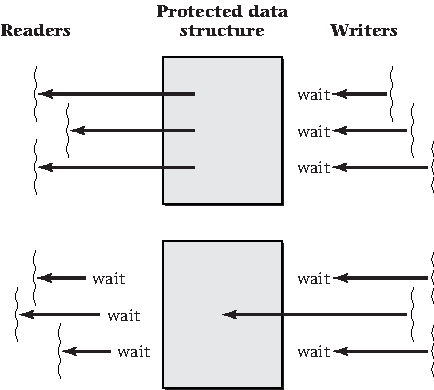
\includegraphics{hail_f0415}}
%\centerline{\epsfbox{scan-4-8.eps}}
\caption{A readers/writers lock can be held either by
  any number of readers or by one writer.  When the lock is held by
  readers, all the reader threads can read the protected data
  structure concurrently.}
\label{scan-4-8}
\end{figure}

Readers/writers locks are particularly valuable in situations where
some of the read-only operations are time consuming, as when reading a
file stored on disk.  This is especially true if many readers are
expected.  The choice between a mutex and a readers/writers lock is a
performance trade-off.  Because the mutex is simpler, it has lower
overhead.  However, the readers/writers lock may pay for its overhead
by allowing more concurrency.

One interesting design question arises if a readers/writers lock is
held by one or more readers and has one or more writers
waiting. Suppose a new reader tries to acquire the lock.  Should it be
allowed to, or should it be forced to wait until after the writers?
On the surface, there seems to be no reason for the reader to wait,
because it can coexist with the existing readers, thereby achieving
greater concurrency.  The problem is that an overlapping succession of
readers can keep the writers waiting arbitrarily long. The writers
could wind up waiting even when the only remaining readers arrived
long after the writers did.  This is a form of \vocab{starvation}, in
that a thread is unfairly prevented from running by other threads.  To
prevent this particular kind of starvation,
some versions of readers/writers locks make new readers wait until
after the waiting writers.

In Section~\ref{condition-variables-section}, you will learn how you
could build readers/writers locks
from more primitive synchronization mechanisms.  However,
because readers/writers locks are so generally useful, they are already
provided by many systems, so you may never actually have to build them
yourself.  The POSIX standard, for example, includes readers/writers
locks with procedures such as \index{pthread_rwlock_init@\verb"|pthread_rwlock_init"|}\verb|pthread_rwlock_init|,
\index{pthread_rwlock_rdlock@\verb"|pthread_rwlock_rdlock"|}\verb|pthread_rwlock_rdlock|, \index{pthread_rwlock_wrlock@\verb"|pthread_rwlock_wrlock"|}\verb|pthread_rwlock_wrlock|, and
\index{pthread_rwlock_unlock@\verb"|pthread_rwlock_unlock"|}\verb|pthread_rwlock_unlock|.  The POSIX standard leaves it up to each
individual system how to prioritize new readers versus waiting
writers.

The POSIX standard also includes a more specialized form of
readers/writers locks specifically associated with files.  This
reflects my earlier comment that readers/writers locking is
especially valuable when reading may be time consuming, as with a file
stored on disk.  In the POSIX standard, file locks are available only
through the complex \index{fcntl@\verb"|fcntl"|}\verb|fcntl| procedure.  However, most UNIX-family
operating systems also provide a simpler interface, \index{flock@\verb"|flock"|}\verb|flock|.

\subsection{Barriers}\label{barriers-section}

\vocabindex{Barrier synchronization}{barrier synchronization}\index{synchronization, barrier} is the last common synchronization pattern I
will discuss.  Barriers are most commonly used in programs that do
large-scale numerical calculations for scientific or engineering
applications, such as simulating ocean currents.  However, they may
also crop up in other applications, as long as there is a requirement
for all threads in a group to finish one phase of the computation
before any of them moves on to the next phase.  In scientific
computations, the threads are often dividing up the processing of a
large matrix.  For example, ten threads may each process 200 rows of a
2000-row matrix.  The requirement for all threads to finish one phase
of processing before starting the next comes from the fact that the
overall computation is a sequence of matrix operations; parallel
processing occurs only within each matrix operation.

When a barrier is created (initialized), the programmer specifies how
many threads will be sharing it.  Each of the threads completes the first
phase of the computation and then invokes the barrier's wait
operation.  For most of the threads, the wait operation does not
immediately return; therefore, the thread calling it cannot
immediately proceed.  The one exception is whichever thread is the
last to call the
wait operation.  The barrier can tell which thread is the last one,
because the programmer specified how many threads there are.  When this last
thread invokes the wait operation, the wait operation immediately
returns.  Moreover, all the other waiting threads finally have their
wait operations also return, as illustrated in Figure~\ref{scan-4-9}.
\begin{figure}
\centerline{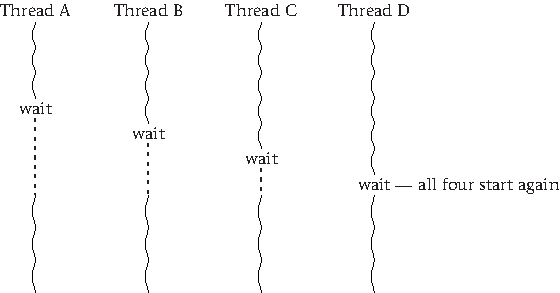
\includegraphics{hail_f0416}}
%\centerline{\epsfbox{scan-4-9.eps}}
\caption{A barrier is created for a specific number of threads.
In this case, there are
  four.  When the last of those threads invokes the wait operation,
  all the waiting threads in the group start running again.}
\label{scan-4-9}
\end{figure}
Thus, they can now all proceed on to the
second phase of the computation.  Typically, the same barrier can then
be reused between the second and third phases, and so forth.  (In other words,
the barrier reinitializes its state once it releases all the waiting
threads.)

Just as with readers/writers locks, you will see how barriers can be
defined in terms of more general synchronization mechanisms.  However,
once again there is little reason to do so in practice, because barriers
are provided as part of POSIX and other widely available APIs.

\section{Condition Variables}\label{condition-variables-section}

In order to solve synchronization problems, such as the three described
in Section~\ref{other-synchronization-problems-section},
you need some mechanism that allows a thread to wait
until circumstances are appropriate for it to proceed.  A producer may
need to wait for buffer space, or a consumer may need to wait for
data.  A reader may need to wait until a writer has unlocked, or a
writer may need to wait for the last reader to unlock.  A thread that
has reached a barrier may need to wait for all the other threads to do
so.  Each situation has its own condition for which a thread must
wait, and there are many other application-specific conditions
besides.  (A video playback that has been paused might wait until the
user presses the pause button again.)

All these examples can be handled by using \vocabs{condition variable}, a
synchronization mechanism that works in partnership with \index{monitor}monitors or
with mutexes used in the style of monitors.  There are two basic
operations on a condition variable: \vocab{wait} and \vocab{notify}.  (Some systems
use the name \vocab{signal} instead of notify.)  A thread that finds
circumstances not to its liking executes the wait operation and
thereby goes to sleep until such time as another thread invokes the
notify operation.  For example, in a bounded buffer, the producer
might wait on a condition variable if it finds the buffer full.  The
consumer, upon freeing up some space in the buffer, would invoke the
notify operation on that condition variable.

Before delving into all the important details and variants,
a concrete example may be helpful.  Figure~\ref{BoundedBuffer.java} shows the Java
code for a \index{BoundedBuffer class@\verb"|BoundedBuffer"|
class}\verb|BoundedBuffer| class.
\begin{figure}
\begin{verbatim}
public class BoundedBuffer {
  private Object[] buffer = new Object[20]; // arbitrary size
  private int numOccupied = 0;
  private int firstOccupied = 0;

  /* invariant: 0 <= numOccupied <= buffer.length
     0 <= firstOccupied < buffer.length
     buffer[(firstOccupied + i) % buffer.length]
     contains the (i+1)th oldest entry,
     for all i such that 0 <= i < numOccupied  */

  public synchronized void insert(Object o)
    throws InterruptedException
  {
    while(numOccupied == buffer.length)
      // wait for space
      wait();
    buffer[(firstOccupied + numOccupied) % buffer.length] = o;
    numOccupied++;
    // in case any retrieves are waiting for data, wake them
    notifyAll();
  }

  public synchronized Object retrieve()
    throws InterruptedException
  {
    while(numOccupied == 0)
      // wait for data
      wait();
    Object retrieved = buffer[firstOccupied];
    buffer[firstOccupied] = null; // may help garbage collector
    firstOccupied = (firstOccupied + 1) % buffer.length;
    numOccupied--;
    // in case any inserts are waiting for space, wake them
    notifyAll();
    return retrieved;
  }
}
\end{verbatim}
\caption{{\tt BoundedBuffer} class using monitors and condition variables}
\label{BoundedBuffer.java}
\end{figure}

Before I explain how this example works, and then return to a more
general discussion of condition variables, you should take a moment to
consider how you would test such a class.  First, it might help to
reduce the size of the buffer, so that all qualitatively different
situations can be tested more quickly.  Second, you need a test program
that has multiple threads doing insertions and retrievals, with some
way to see the difference between when each operation is started and
when it completes.  In the case of the retrievals, you will also need
to see that the retrieved values are correct.  Designing such a test
program is surprisingly interesting; you can have this experience in Programming Project~\ref{bounded-buffer-test-project}.

In Java, each object has a single condition variable automatically
associated with it, just as it has a mutex.  The \index{wait@\verb"|wait"|}\verb|wait| method
waits on the object's condition variable, and the \index{notifyAll@\verb"|notifyAll"|}\verb|notifyAll|
method wakes up all threads waiting on the object's condition
variable.  Both of these methods need to be called by a thread that
holds the object's mutex.  In my \verb|BoundedBuffer| example, I
ensured this in a straightforward way by using \verb|wait| and
\verb|notifyAll| inside methods that are marked \verb|synchronized|.

Having seen that \verb|wait| and \verb|notifyAll| need to be called
with the mutex held, you may spot a problem.  If a waiting thread
holds the mutex, there will be no way for any other thread to acquire
the mutex, and thus be able to call \verb|notifyAll|.  Until you learn
the rest of the story, it seems as though any thread that invokes
\verb|wait| is doomed to eternal waiting.

The solution to this dilemma is as follows.  When a thread invokes the
wait operation, it must hold the associated mutex.  However, the wait
operation releases the mutex before putting the thread into its
waiting state.  That way, the mutex is available to a potential waker.
When the waiting thread is awoken, it reacquires the mutex before the
wait operation returns.  (In the case of recursive mutexes, as used in
Java, the awakening thread reacquires the mutex with the same lock
count as before, so that it can still do just as many unlock
operations.)

The fact that a waiting thread temporarily releases the mutex helps
explain two features of the \verb|BoundedBuffer| example.  First, the waiting
is done at the very beginning of the methods.  This ensures that the
invariant is still intact when the mutex is released.  (More
generally, the waiting could happen later, as long as no state
variables have been updated, or even as long as they have been put
back into an invariant-respecting state.)  Second, the waiting is done
in a loop; only when the waited-for condition has been verified to
hold does the method move on to its real work.  The loop is essential
because an awoken thread needs to reacquire the mutex, contending with
any other threads that are also trying to acquire the mutex.  There is
no guarantee that the awoken thread will get the mutex first.  As
such, there is no guarantee what state it will find; it may need to
wait again.

When a waiting thread releases the mutex in order to wait on the
condition variable, these two actions are done indivisibly.  There is
no way another thread can acquire the mutex before the first thread
has started waiting on the condition variable.  This ensures no other
thread will do a notify operation until after the thread that wants to
wait is actually waiting.

In addition to waiting for appropriate conditions at the top of each
method, I have invoked \verb|notifyAll| at the end of each
method.  This position is less crucial, because the \verb|notifyAll|
method does not release the mutex.  The calling thread continues to
hold the mutex until it reaches the end of the synchronized method.
Because an awoken thread needs to reacquire the mutex, it will not be
able to make any headway until the notifying method finishes,
regardless of where in that method the notification is done.

One early version of monitors with condition variables (as described by
\index{Hoare, C. A. R.@Hoare, C.~A.~R.}Hoare) used a different approach.  The notify operation immediately
transferred the mutex to the awoken thread, with no contention from
other waiting threads.  The thread performing the notify operation
then waited until it received the mutex back from the awoken thread.
Today, however, the version I described previously seems to be
dominant.  In particular, it is used not only in Java, but also in the
POSIX API.

The \verb|BoundedBuffer| code in Figure~\ref{BoundedBuffer.java}
takes a very aggressive approach to notifying waiting threads: at the
end of any operation all waiting threads are woken using
\verb|notifyAll|.  This is a very safe approach; if the
\verb|BoundedBuffer|'s state was changed in a way of interest to any thread,
that thread will be sure to notice.  Other threads that don't care can
simply go back to waiting.  However, the program's efficiency may be improved
somewhat by reducing the amount of notification done.
Remember, though, that correctness should always
come first, with optimization later, if at all.  Before optimizing,
check whether the simple, correct version actually performs
inadequately.

There are two approaches to reducing notification.  One is to put the
\verb|notifyAll| inside an \verb|if| statement, so that it is done
only under some circumstances, rather than unconditionally.  In
particular, producers should be waiting only if the buffer is full,
and consumers should be waiting only if the buffer is empty.
Therefore, the only times when notification is needed are when
inserting into an empty buffer or retrieving from a full buffer.  In
Programming Project~\ref{conditional-notifyAll-project}, you can modify the code to reflect this and test that it
still works.

The other approach to reducing notification is to use the
\index{notify@\verb"|notify"|}\verb|notify| method in place of \verb|notifyAll|.  This way, only a
single waiting thread is awoken, rather than all waiting threads.
Remember that optimization should be considered only if
the straightforward version performs inadequately.  This cautious
attitude is appropriate because programmers find it rather tricky to
reason about whether
\verb|notify| will suffice.  As such, this optimization is quite error-prone.
In
order to verify that the change from \verb|notifyAll| to \verb|notify|
is correct, you need to check two
things:
\begin{enumerate}
\item
There is no danger of waking too few threads.  Either you have some way
to know that only one is waiting, or you know that only one would be
able to proceed, with the others looping back to waiting.
\item
There is no danger of waking the wrong thread.  Either you have some
way to know that only one is waiting, or you know that all are equally
able to proceed.  If there is any thread which could proceed if it got
the mutex first, then all threads have that property.  For example, if
all the waiting threads are executing the identical while loop, this
condition will be satisfied.
\end{enumerate}
In
Exercise~\ref{notify-exercise}, you can show that these two conditions do not hold for the \verb|BoundedBuffer|
example: replacing \verb|notifyAll| by \verb|notify| would not be safe
in this case.  This is true even if the notification operation is
done unconditionally, rather than inside an \verb|if| statement.

One limitation of Java is that each object has only a single condition
variable.  In the \verb|BoundedBuffer| example, any thread waits on that one
condition variable, whether it is waiting for space in the
\verb|insert| method or for data in the \verb|retrieve| method.  In a
system which allows multiple condition variables to be associated with
the same monitor (or mutex), you could use two different condition
variables.  That would allow you to specifically notify a thread
waiting for space (or one waiting for data).

The POSIX API allows multiple condition variables per mutex.
In Programming Project~\ref{bb-two-condvars-project} you can use this
feature to rewrite the \verb|BoundedBuffer| example with
two separate condition variables, one used to wait for space and the
other used to wait for data.

POSIX condition variables are initialized with \index{pthread_cond_init@\verb"|pthread_cond_init"|}\verb|pthread_cond_init|
independent of any particular mutex; the mutex is instead passed as an
argument to \index{pthread_cond_wait@\verb"|pthread_cond_wait"|}\verb|pthread_cond_wait|, along with the condition
variable being waited on.  This is a somewhat error-prone arrangement,
because all concurrent waiters need to pass in the same mutex.  The
operations corresponding to \verb|notify| and \verb|notifyAll| are
called \index{pthread_cond_signal@\verb"|pthread_cond_signal"|}\verb|pthread_cond_signal| and \index{pthread_cond_broadcast@\verb"|pthread_cond_broadcast"|}\verb|pthread_cond_broadcast|.
The API allows a thread to invoke
\verb|pthread_|\linebreak[0]\verb|cond_signal| or \verb|pthread_cond_broadcast|
without holding a corresponding mutex, but using this
flexibility without introducing a race bug is difficult.

The same technique I illustrated with \verb|BoundedBuffer| can be applied
equally well for readers/writers locks or barriers; I leave these as
Programming Projects \ref{rw-project} and \ref{barrier-project}.  More importantly, the same technique will also work for
application-specific synchronization needs.  For example, a video
player might have a state variable that indicates whether the player is
currently paused.  The playback thread checks that variable before
displaying each frame, and if paused, waits on a condition variable.
The user-interface thread sets the variable in response to the user
pressing the pause button.  When the user interface puts the variable
into the unpaused state, it does a notify operation on the condition
variable.  You can develop an application analogous to this in
Programming Project~\ref{simulator-synchronization-project}.

\section{Semaphores}\label{semaphores-section}

You have seen that monitors with condition variables are quite general
and can be used to synthesize other more special-purpose
synchronization mechanisms, such as readers/writers locks.  Another
synchronization mechanism with the same generality is the semaphore.
For most purposes, semaphores are less natural, resulting in more
error-prone code.  In those applications where they are natural (for
example, bounded buffers), they result in very succinct, clear code.
That is probably not the main reason for their continued use, however.
Instead, they seem to be hanging on largely out of historical inertia,
having gotten a seven- to nine-year head start over monitors.  (Semaphores date to 1965,
as opposed to the early 1970s for monitors.)

A \vocab{semaphore} is essentially an unsigned integer variable, that is, a
variable that can take on only nonnegative integer values.  However,
semaphores may not be freely operated on with arbitrary arithmetic.
Instead, only three operations are allowed:
\begin{itemize}
\item
At the time the semaphore is created, it may be initialized to any
nonnegative integer of the programmer's choice.
\item
A semaphore may be increased by 1.  The operation to do this is
generally called either \index{release@\verb"|release"|}\verb|release|, \index{up@\verb"|up"|}\verb|up|, or \index{V@\verb"|V"|}\verb|V|.  The letter \verb|V| is short
for a Dutch word that made sense to \index{Dijkstra, Edsger W.}Dijkstra, the 1965 originator of
semaphores.  I will use \verb|release|.
\item
A semaphore may be decreased by 1.  The operation to do this is
frequently called either \index{acquire@\verb"|acquire"|}\verb|acquire|, \index{down@\verb"|down"|}\verb|down|, or \index{P@\verb"|P"|}\verb|P|.  Again, \verb|P| is
a Dutch abbreviation.  I will use \verb|acquire|.  Because the
semaphore's value must stay nonnegative, the thread performing an
\verb|acquire| operation waits if the value is 0.  Only once another
thread has performed a \verb|release| operation to make the value positive
does the waiting thread continue with its \verb|acquire| operation.
\end{itemize}

One common use for semaphores is as mutexes.
If a semaphore is initialized to 1, it can serve as a mutex,
with \verb|acquire| as the locking operation and \verb|release| as the
unlocking operation.  Assuming that locking and unlocking are properly
paired, the semaphore will only ever have the values 0 and 1.  When it
is locked, the value will be 0, and any further attempt to lock it
(using \verb|acquire|) will be forced to wait.  When it is is unlocked,
the value will be 1, and locking can proceed.  Note, however, that
semaphores used in this limited way have no advantage over mutexes.
Moreover, if a program bug results in an attempt to unlock an already
unlocked mutex, a special-purpose mutex could signal the error,
whereas a general-purpose semaphore will simply increase to 2, likely
causing nasty behavior later when two threads are both allowed to execute
\verb|acquire|.

A better use for semaphores is for keeping track of the available
quantity of some resource, such as free spaces or
data values in a bounded buffer. Whenever a thread creates a unit of
the resource, it increases the semaphore.  Whenever a thread wishes to
consume a unit of the resource, it first does an \verb|acquire| operation
on the semaphore.  This both forces the thread to wait until at least
one unit of the resource is available and stakes the thread's claim to
that unit.

Following this pattern, the \index{BoundedBuffer class@\verb"|BoundedBuffer"| class}\verb|BoundedBuffer| class can be
  rewritten to use
semaphores, as shown in Figure~\ref{SemaphoreBoundedBuffer.java}.
\begin{figure}
\begin{verbatim}
import java.util.concurrent.Semaphore;

public class BoundedBuffer {
  private java.util.List<Object> buffer =
    java.util.Collections.synchronizedList
    (new java.util.LinkedList<Object>());

  private static final int SIZE = 20; // arbitrary

  private Semaphore occupiedSem = new Semaphore(0);
  private Semaphore freeSem = new Semaphore(SIZE);

  /* invariant: occupiedSem + freeSem = SIZE
     buffer.size() = occupiedSem
     buffer contains entries from oldest to youngest */

  public void insert(Object o) throws InterruptedException{
    freeSem.acquire();
    buffer.add(o);
    occupiedSem.release();
  }

  public Object retrieve() throws InterruptedException{
    occupiedSem.acquire();
    Object retrieved = buffer.remove(0);
    freeSem.release();
    return retrieved;
  }
}
\end{verbatim}
\caption{Alternative {\tt BoundedBuffer} class, using semaphores}
\label{SemaphoreBoundedBuffer.java}
\end{figure}
This uses the a class of semaphores imported from one of the
packages of the Java API, \texttt{java.util.concurrent}.
In
Programming Project~\ref{semaphore-project}, you can instead write your own {\tt Semaphore} class using Java's built-in mutexes and
condition variables.

In order to show semaphores in the best possible light, I also moved
away from using an array to store the buffer.  Instead, I used a
\texttt{List}, provided by the Java API.  If, in Programming Project~\ref{semaphore-array-bb-project}, you try rewriting
this example to use an array (as in Figure~\ref{BoundedBuffer.java}),
you will discover two blemishes.  First, you will need the
\verb|numOccupied| integer variable, as in Figure~\ref{BoundedBuffer.java}.  This duplicates the information contained in
\verb|occupiedSem|, simply in a different form.  Second, you will need
to introduce explicit mutex synchronization with \verb|synchronized|
statements around the code that updates the nonsemaphore state
variables.  With those complications, semaphores lose some of their
charm.  However, by using a \texttt{List}, I hid the extra complexity.

\section{Deadlock}\label{deadlock-section}

In Chapter~\ref{threads-chapter}, I introduced concurrency as a way to solve
problems of responsiveness and throughput.  Unfortunately, concurrency
created its own problem---races.  Therefore, I introduced
synchronization to solve the problem of races.  The obvious question is, what new problems arise
from synchronization?  One easy answer is that synchronization has
reintroduced the original responsiveness and throughput problems to some lesser degree, because
synchronization reduces concurrency.  However, as you will see in this
section, synchronization also creates an entirely new problem, and one that is
potentially more serious.  Section~\ref{deadlock-problem-section}
explains this problem, known as deadlock, whereby threads can wind up
permanently waiting.  Sections
\ref{deadlock-prevention-section} through \ref{immediate-dd-section}
explain three different solutions to the problem.

\subsection{The Deadlock Problem}\label{deadlock-problem-section}

To illustrate what a deadlock is, and how one can arise,
consider a highly simplified system for keeping bank accounts.
Suppose each account is an object with two components: a mutex and a
current balance.  A procedure for transferring money from one account
to another might look as follows, in pseudocode:
\begin{verbatim}
to transfer amount from sourceAccount to destinationAccount:
  lock sourceAccount.mutex
  lock destinationAccount.mutex
  sourceAccount.balance = sourceAccount.balance - amount
  destinationAccount.balance = destinationAccount.balance + amount
  unlock sourceAccount.mutex
  unlock destinationAccount.mutex
\end{verbatim}

Suppose I am feeling generous and transfer \$100 from \verb|myAccount|
to \verb|yourAccount|.  Suppose you are feeling even more generous
and transfer \$250 from \verb|yourAccount| to \verb|myAccount|.  With
any luck, at the end I should be \$150 richer and you should be \$150
poorer.  If either transfer request is completed before the other
starts, this is exactly what happens.  However, what if the two execute
concurrently?

The mutexes prevent any race condition, so you can be sure that the
accounts are not left in an inconsistent state.  Note that we have
locked both accounts for the entire duration of the transfer, rather
than locking each only long enough to update its balance.  That way, an
auditor can't see an alarming situation where money has disappeared
from one account but not yet appeared in the other account.

However, even though there is no race, not even with an auditor, all is not
well.  Consider the following sequence of events:
\begin{enumerate}
\item
I lock the source account of my transfer to you.  That is, I lock
\verb|myAccount.mutex|.
\item
You lock the source account of your transfer to me.  That is, you lock
\verb|yourAccount.mutex|.
\item
I try to lock the destination account of my transfer to you.  That is,
I try to lock \verb|yourAccount.mutex|.  Because you already hold this
mutex, I am forced to wait.
\item
You try to lock the destination account of your transfer to me.  That is,
you try to lock \verb|myAccount.mutex|.  Because I already hold this
mutex, you are forced to wait.
\end{enumerate}
At this point, each of us is waiting for the other: we have
deadlocked.

More generally, a \vocab{deadlock} exists whenever there is a cycle of
threads, each waiting for some resource held by the next.  In the
example, there were two threads and the resources involved were two
mutexes.  Although deadlocks can involve other resources as well
(consider readers/writers locks, for example), I will focus
on mutexes for simplicity.

As an example of a deadlock involving more than two threads, consider
generalizing the preceding scenario of transferring money between bank accounts.
Suppose, for example, that there are five bank accounts, numbered 0
through 4.  There are also five threads.  Each thread is trying to
transfer money from one account to another, as shown in
Figure~\ref{deadlocking-transfers-table}.
\begin{figure}
\centerline{\begin{tabular}{|c|c|c|}
\hline\bf Thread & \bf Source Account & \bf Destination Account\\\hline
0 & 0 & 1\\\hline
1 & 1 & 2\\\hline
2 & 2 & 3\\\hline
3 & 3 & 4\\\hline
4 & 4 & 0\\\hline
\end{tabular}}
\caption{Each of five threads tries to transfer money from a source
  account to a destination account.  If each thread locks its
  source account, none will be able to proceed by locking its
  destination account.}\label{deadlocking-transfers-table}
\end{figure}
As before, each transfer
involves locking the source and destination accounts.  Once again, the
threads can deadlock if each one locks the source account first, and
then tries to lock the destination account.  This situation is much
more famous when dressed up as the \index{dining philosophers}dining
philosophers problem, which I describe next.

In 1972, \index{Dijkstra, Edsger W.}Dijkstra wrote about a group of five philosophers, each of
whom had a place at a round dining table, where they ate a
particularly difficult kind of spaghetti that required two forks.
There were five forks at the table, one between each pair of
adjacent plates, as shown in Figure~\ref{dining-figure}.
\begin{figure}
\centerline{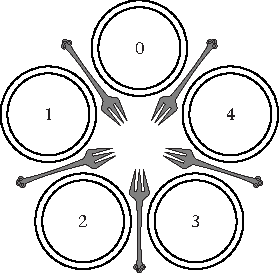
\includegraphics{hail_f0420}}
%\centerline{\epsfbox{dining.eps}}
\caption{Five philosophers, numbered 0 through 4, have places around a
  circular dining table.  There is a fork between each pair of
  adjacent places.  When each philosopher tries to pick up two forks,
  one at a time,
  deadlock can result.}
\label{dining-figure}
\end{figure}
Apparently
Dijkstra was not concerned with communicable diseases such as
mononucleosis, because he thought it was OK for the philosophers
seated to the left and right of a particular fork to share it.
Instead, he was concerned with the possibility of deadlock.  If all five philosophers start by
picking up their respective left-hand forks and then wait for their right-hand forks to become available, they wind up deadlocked.
In
Exploration Project~\ref{dining-philosophers-project}, you can try out
a computer simulation of the dining philosophers.  In that same Exploration
Project, you can also apply the deadlock prevention approach described
in Section~\ref{deadlock-prevention-section} to the dining
philosophers problem.

Deadlocks are usually quite rare even if no special attempt is made
to prevent them, because most locks are not held very long.  Thus,
the window of opportunity for deadlocking is quite narrow, and, like
races, the timing must be exactly wrong.  For a very noncritical system,
one might choose to ignore the possibility of deadlocks.  Even if the
system needs the occasional reboot due to deadlocking, other
malfunctions will probably be more common.  Nonetheless, you should
learn some options for dealing with deadlocks, both because some
systems are critical and because ignoring a known problem is
unprofessional.  In Sections \ref{deadlock-prevention-section} through
\ref{immediate-dd-section}, I explain three of the
most practical ways to address the threat of deadlocks.

\subsection{Deadlock Prevention Through Resource Ordering}\label{deadlock-prevention-section}

The ideal way to cope with deadlocks is to prevent them from
happening.  One very practical technique for deadlock prevention can
be illustrated through the example of transferring money between two bank accounts.
Each of the two accounts is stored somewhere in the computer's
memory, which can be specified through a numerical address.  I will
use the notation \verb|min(account1, account2)| to mean whichever of
the two account objects occurs at the lower address (earlier in
memory). Similarly, I will use \verb|max(account1, account2)| to mean
whichever occurs at the higher address.  I can use this ordering on
the accounts (or any other ordering, such as by account number) to
make a deadlock-free transfer procedure:
\begin{verbatim}
to transfer amount from sourceAccount to destinationAccount:
  lock min(sourceAccount, destinationAccount).mutex
  lock max(sourceAccount, destinationAccount).mutex
  sourceAccount.balance = sourceAccount.balance - amount
  destinationAccount.balance = destinationAccount.balance + amount
  unlock sourceAccount.mutex
  unlock destinationAccount.mutex
\end{verbatim}

Now if I try transferring money to you, and you try transferring money
to me, we will both lock the two accounts' mutexes in the same order.
No deadlock is possible; one transfer will run to completion, and then
the other.

The same technique can be used whenever all the mutexes (or other
resources) to be acquired are known in advance.  Each thread should
acquire the resources it needs in an agreed-upon order, such as by
increasing memory address.  No matter how many threads and resources
are involved, no deadlock can occur.

As one further example of this technique, you can look at some code
from the Linux kernel.  Recall from Chapter~\ref{scheduling-chapter} that the scheduler keeps the run queue,
which holds runnable
threads, in a data structure.  In the kernel
source code, this structure is
known as an \texttt{rq}.  Each processor in a multiprocessor system has
its own \texttt{rq}.  When the scheduler moves a thread from one processor's
\texttt{rq} to another's, it needs to lock both \texttt{rq}s.
Figure~\ref{double_rq_lock} shows the code to
do this.  Note that this
procedure uses the deadlock prevention technique with one refinement:
it also tests for the special case that the two runqueues are
in fact one and the same.
\begin{figure}
%examplesource: linux-2.6.39/kernel/sched.c
%exampleedit: indentation increment reduced to fit margin
\begin{verbatim}
static void double_rq_lock(struct rq *rq1, struct rq *rq2)
  __acquires(rq1->lock)
  __acquires(rq2->lock)
{
  BUG_ON(!irqs_disabled());
  if (rq1 == rq2) {
    raw_spin_lock(&rq1->lock);
    __acquire(rq2->lock);   /* Fake it out ;) */
  } else {
    if (rq1 < rq2) {
      raw_spin_lock(&rq1->lock);
      raw_spin_lock_nested(&rq2->lock, SINGLE_DEPTH_NESTING);
    } else {
      raw_spin_lock(&rq2->lock);
      raw_spin_lock_nested(&rq1->lock, SINGLE_DEPTH_NESTING);
    }
  }
}
\end{verbatim}
\caption{The Linux scheduler uses deadlock prevention when locking two
run queues.}
\label{double_rq_lock}
\end{figure}

Deadlock prevention is not always possible.  In particular, the
ordering technique I showed cannot be used if the mutexes that need
locking only become apparent one by one as the computation proceeds,
such as when following a linked list or other pointer-based
data structure.  Thus, you need to consider coping with deadlocks,
rather than only preventing them.

\subsection{Ex Post Facto Deadlock Detection}\label{post-facto-dd-section}
\index{deadlock detection}
In order to diagnose deadlocks, you need some information about who is
waiting for whom.  Suppose that each mutex records not just whether it
is locked or unlocked, but also which thread it is held by, if any.
(This information may be useful for unrelated purposes as well, such
as implementing recursive or error-checking mutexes.)  Additionally,
when a thread is unable to immediately acquire a mutex and is put
into a waiting state, you can record which mutex it is waiting for.
With this information, you can construct a \vocab{resource allocation graph}.
Figure~\ref{resource-allocation-graph} shows an example graph for
Section~\ref{deadlock-problem-section}'s sample deadlock between bank account transfers.
Squares are threads and circles are mutexes.  The arrows show which
mutex each thread is waiting to acquire and which thread each mutex
is currently held by.
Because the graph has a cycle, it shows that the system is deadlocked.
\begin{figure}
\centerline{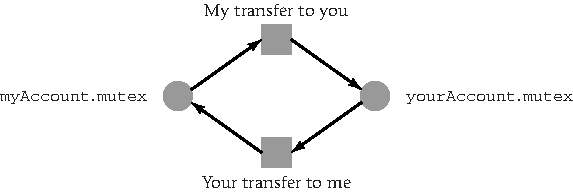
\includegraphics{hail_f0422}}
\iffalse
\centerline{\begin{graph}(294,94)(-43,3)
\graphnodesize{10}
\graphlinecolour{0}
\graphlinewidth{0.5}
\grapharrowlength{5}
\graphnodecolour{0}
\fillednodestrue
\roundnode{myMutex}(50,50)
\roundnode{yourMutex}(150,50)
\squarenode{myTransfer}(100,80)
\squarenode{yourTransfer}(100,20)
\autonodetext{myMutex}[w]{myAccount.mutex}
\autonodetext{yourMutex}[e]{yourAccount.mutex}
\autonodetext{myTransfer}[n]{my transfer to you}
\autonodetext{yourTransfer}[s]{your transfer to me}
\diredge{myTransfer}{yourMutex}
\diredge{yourMutex}{yourTransfer}
\diredge{yourTransfer}{myMutex}
\diredge{myMutex}{myTransfer}
\end{graph}}
\fi
\caption{The cycle in this resource allocation graph indicates a
  deadlock.  Each square represents a thread and each circle a mutex.
  An arrow from a square to a circle shows a thread waiting for a
  mutex, whereas an arrow from a circle to a square shows a mutex
  being held by a thread.}
\label{resource-allocation-graph}
\end{figure}

A system can test for deadlocks periodically or when a thread has
waited an unreasonably long time for a lock.  In order to test for a
deadlock, the system uses a standard graph algorithm to check whether
the resource allocation graph contains a cycle. With the sort of
mutexes described in this book, each mutex can be held by at most
one thread and each thread is waiting for at most one mutex, so no
vertex in the graph has an out-degree greater than 1.  This allows a
somewhat simpler graph search than in a fully-general directed graph.

Once a deadlock is detected, a painful action is needed in order to
recover: one of the deadlocked threads must be forcibly terminated, or
at least rolled back to an earlier state, so as to free up the
mutexes it holds.  In a general computing environment, where threads
have no clean way to be rolled back, this is bit akin to freeing
yourself from a bear trap by cutting off your leg.  For this reason,
ex post facto deadlock detection is not common in general-purpose
operating systems.

One environment in which ex post facto deadlock detection and recovery
works cleanly is database systems, with their support for atomic
transactions.  I will explain atomic transactions in Chapter~\ref{transactions-chapter};
for now, you need only understand that a transaction can
cleanly be rolled back, such that all the updates it made to the
database are undone.  Because this infrastructure is available,
database systems commonly include deadlock detection.  When a deadlock
is detected, one of the transactions fails and can be rolled back,
undoing all its effects and releasing all its locks.  This breaks the
deadlock and allows the remaining transactions to complete.  The
rolled-back transaction can then be restarted.

Figure~\ref{oracle-deadlock} shows an example scenario of deadlock
detection taken from the Oracle database system.
This transcript shows the time interleaving of two
different sessions connected to the same database.  One session is
shown at the left margin, while the other session is shown indented
four spaces.  Command lines start with the system's prompt,
\texttt{SQL>}, and then contain a command typed by the user.  Each
command line is broken on to a second line, to fit the width of this
book's pages.
Explanatory comments start with \texttt{-{}-}.  All other lines are
output.
In Chapter~\ref{transactions-chapter} I will show the recovery from this particular
deadlock as part of my explanation of transactions.
\begin{figure}
%Note that I've taken liberties with when the SQL> prompt is displayed,
%always putting it where the command is being entered, rather than when
%it was actually displayed (eariler).  I've also had to break lines.
\begin{verbatim}
SQL> update accounts set balance = balance - 100
                     where account_number = 1;

1 row updated.

    SQL> update accounts set balance = balance - 250
                         where account_number = 2;

    1 row updated.

SQL> update accounts set balance = balance + 100 
                         where account_number = 2;
-- note no response, for now this SQL session is hanging

    SQL> update accounts set balance = balance + 250 
                         where account_number = 1;
    -- this session hangs, but in the other SQL session we get
    -- the following error message:

update accounts set balance = balance + 100 
                where account_number = 2
       *
ERROR at line 1:
ORA-00060: deadlock detected while waiting for resource 
\end{verbatim}
\caption{The Oracle database
  system detects a deadlock between two sessions connected to the same
  database.  One session, shown at the left margin, is transferring \$100
  from account 1 to account 2.  The other session, shown indented, is
  transferring \$250 from account 2 to account 1.  Each update statement
  locks the account being updated.  Therefore, each session hangs when it
  tries locking the account that the other session has previously locked.}
\label{oracle-deadlock}
\end{figure}

\subsection{Immediate Deadlock Detection}\label{immediate-dd-section}

The two approaches to deadlocks presented thus far are aimed
at the times before and after the moment when deadlock occurs.  One
arranges that the prerequisite circumstances leading to deadlock do
not occur, while the other notices that deadlock already has occurred,
so that the mess can be cleaned up.  Now I will turn to a third
alternative: intervening at the very moment when the system would
otherwise deadlock.  Because this intervention requires techniques similar to those discussed in Section~\ref{post-facto-dd-section}, this technique is conventionally known
as a form of deadlock detection rather than deadlock prevention, even
though from a literal perspective the deadlock is prevented from
happening.

As long as no deadlock is ever allowed to occur, the resource
allocation graph will remain acyclic, that is, free of cycles.  Each time a thread tries to
lock a mutex, the system can act as follows:
\begin{itemize}
\item
If the mutex is unlocked, lock it and add an edge from the mutex to
the thread, so as to indicate which thread now holds the lock.
\item
If the mutex is locked, follow the chain of edges from it until that
chain dead ends.  (It must, because the graph is acyclic.)  Is the end
of the chain the same as the thread trying to lock the mutex?
\begin{itemize}
\item
If not, add an edge showing that the thread is waiting for the mutex,
and put the thread into a waiting state.
\item
If the end of the chain is the same thread, adding the extra edge would complete a cycle, as shown in
Figure~\ref{idd-rg-figure}.
\begin{figure}
\centerline{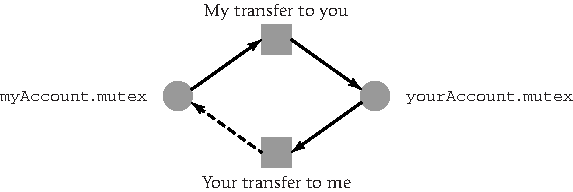
\includegraphics{hail_f0424}}
\iffalse
\centerline{\begin{graph}(294,94)(-43,3)
\graphnodesize{10}
\graphlinecolour{0}
\graphlinewidth{0.5}
\grapharrowlength{5}
\graphnodecolour{0}
\fillednodestrue
\roundnode{myMutex}(50,50)
\roundnode{yourMutex}(150,50)
\squarenode{myTransfer}(100,80)
\squarenode{yourTransfer}(100,20)
\autonodetext{myMutex}[w]{myAccount.mutex}
\autonodetext{yourMutex}[e]{yourAccount.mutex}
\autonodetext{myTransfer}[n]{my transfer to you}
\autonodetext{yourTransfer}[s]{your transfer to me}
\diredge{myTransfer}{yourMutex}
\diredge{yourMutex}{yourTransfer}
\diredge{yourTransfer}{myMutex}[\graphlinedash{1 2}]
\diredge{myMutex}{myTransfer}
\end{graph}}
\fi
\caption{In this resource graph, the solid arrows indicate that my
  transfer holds {\tt myAccount.mutex}, your transfer holds {\tt
  yourAccount.mutex}, and my transfer is waiting for {\tt
  yourAccount.mutex}.  The dashed arrow indicates a request currently
  being made by your transfer to lock {\tt myAccount.mutex}. If this
  dashed arrow is added, a
  cycle is completed, indicating a deadlock.  Therefore, the request
  will fail rather than enter a state of waiting.}
\label{idd-rg-figure}
\end{figure}
Therefore, don't add the edge, and don't put
the thread into a waiting state.  Instead, return an error code from the
lock request (or throw an exception), indicating that the mutex could
not be locked because a deadlock would have resulted.
\end{itemize}
\end{itemize}

Notice that the graph search here is somewhat simpler than in
ex post facto deadlock detection, because the graph is kept acyclic.
Nonetheless, the basic idea is the same as deadlock detection, just
done proactively rather than after the fact.  As with any deadlock
detection, some form of roll-back is needed; the application program
that tried to lock the mutex must respond to the news that its request
could not be granted.  The application program must not simply try
again to acquire the same mutex, because it will repeatedly get the
same error code.  Instead, the program must release the locks it
currently holds and then restart from the beginning.  The chance of
needing to repeat this response can be reduced by sleeping briefly
after releasing the locks and before restarting.

Designing an application program to correctly handle immediate
deadlock detection can be challenging.  The difficulty is that before
the program releases its existing locks, it should restore the objects
those locks were protecting to a consistent state.  One case in which
immediate deadlock detection can be used reasonably easily is in a
program that acquires all its locks before it modifies any objects.

One example of immediate deadlock detection is in
Linux and Mac OS~X, for the readers/writers locks placed on files using
\index{fcntl@\verb"|fcntl"|}\verb|fcntl|.  If a lock request would complete a cycle, the
\verb|fcntl| procedure returns the error code \index{EDEADLK@\verb"|EDEADLK"|}\verb|EDEADLK|.  However, this
deadlock detection is not a mandatory part of the POSIX specification
for \verb|fcntl|.

\section{The Interaction of Synchronization with Scheduling}\label{synchronization-and-scheduling-section}

Recall that the scheduler controls which runnable thread runs on each processor, and
synchronization actions performed by the running thread control which
threads are runnable.  Therefore, synchronization and scheduling interact with one another.
Two forms of interaction, known as priority inversion and the convoy
phenomenon, are particularly interesting.  Said another way, they can
cause lots of grief.  Each can subvert the prioritization of threads,
and the convoy phenomenon can also greatly increase the context
switching rate and hence decrease system throughput.
For simplicity, each is presented here under the assumption of a single-processor system.

\subsection{Priority Inversion}

When a priority-based scheduler is used, a high-priority thread should
not have to wait while a low-priority thread runs.  If threads of
different priority levels share mutexes or other blocking synchronization
primitives, some minor violations of priority ordering are
inevitable.  For example, consider the following sequence of events
involving two threads (high-priority and low-priority) that share a
single mutex:
\begin{enumerate}
\item
The high-priority thread goes into the waiting state, waiting for an
I/O request to complete.
\item
The low-priority thread runs and acquires the mutex.
\item
The I/O request completes, making the high-priority thread runnable
again.  It preempts the low-priority thread and starts running.
\item
The high-priority thread tries to acquire the mutex.  Because the mutex
is locked, the high-priority thread is forced to wait.
\item
The low-priority thread resumes running.
\end{enumerate}
At this point, a high-priority thread is waiting while a low-priority
thread runs.  However, this temporary violation of priority ordering
is not a big deal, because programmers generally ensure that no thread
holds a mutex for very long.  As such, the low-priority thread will
soon release the mutex and allow the high-priority thread to run.

However, another, more insidious problem can lead to longer-term
violation of priority order (that is, \foldvocab{priority}{inversion}).  Suppose
there are three threads, of low, medium, and high priority.  Consider this
sequence of events:
\begin{enumerate}
\item
The high- and medium-priority threads both go into the waiting state,
each waiting for an I/O request to complete.
\item
The low-priority thread runs and acquires the mutex.
\item
The two I/O requests complete, making the high- and medium-priority
threads runnable.  The high-priority thread preempts the low-priority
thread and starts running.
\item
The high-priority thread tries to acquire the mutex.  Because the mutex
is locked, the high-priority thread is forced to wait.
\item
At this point, the medium-priority thread has the highest priority of
those that are runnable.  Therefore it runs.
\end{enumerate}

In this situation, the medium-priority thread is running and
indirectly keeping the high-priority thread from running.  (The
medium-priority thread is blocking the low-priority thread by virtue
of their relative priorities.  The low-priority thread is blocking the
high-priority thread by holding the mutex.)  The medium-priority
thread could run a long time.  In fact, a whole succession of
medium-priority threads with overlapping lifetimes could come and
go, and the high-priority thread would wait the whole time despite its
higher priority.  Thus, the priority inversion could continue for an arbitrarily long time.

One ``solution'' to the priority inversion problem is to avoid
fixed-priority scheduling.  Over time, a decay usage scheduler will
naturally lower the priority of the medium-priority thread that is
running.  Eventually it will drop below the low-priority thread, which
will then run
and free the mutex, allowing the high-priority thread to run.
However, a succession of medium-priority threads, none of which runs
for very long, could still hold up the high-priority thread
arbitrarily long.  Therefore, Microsoft Windows responds to priority
inversion by periodically boosting the priority of waiting low-priority processes.

This first ``solution'' has two shortcomings.  First, it may be sluggish in
responding to a priority inversion.  Second, fixed-priority scheduling
is desirable in some applications, such as real-time systems.
Therefore, a genuine solution to the priority inversion
problem is needed---one that makes the problem go away, rather than just
limiting the duration of its effect.  The genuine solution is
\foldvocab{priority}{inheritance}.

Priority inheritance is a simple idea: any thread that is waiting for
a mutex temporarily ``lends'' its priority to the thread that holds
the mutex.  A thread that holds mutexes runs with the highest priority
among its own priority and those priorities it has been lent by threads waiting for the
mutexes.  In the example with three threads, priority inheritance will allow the low-priority thread that
holds the mutex to run as though it were high-priority until it
unlocks the mutex.  Thus, the truly high-priority thread will get to
run as soon as possible, and the medium-priority thread will have to
wait.

Notice that the high-priority thread has a very selfish motive for
letting the low-priority thread use its priority: it wants to get the
low-priority thread out of its way.  The same principle can be applied
with other forms of scheduling than priority scheduling.  By analogy
with priority inheritance, one can have \foldvocab{deadline}{inheritance} (for
Earliest Deadline First scheduling) or even a lending of processor
allocation shares (for proportional-share scheduling).

\subsection{The Convoy Phenomenon}\label{convoy-section}

I have remarked repeatedly that well-designed programs do not
normally hold any mutex for very long; thus, attempts to lock a mutex
do not normally encounter contention.  This is important because
locking a mutex with contention is much more expensive.  In
particular, the big cost of a request to lock an already-locked mutex
is context switching, with the attendant loss of cache performance.
Unfortunately, one particularly nasty interaction between scheduling
and synchronization, known as the \vocab{convoy phenomenon}, can sometimes
cause a heavily used mutex to be perpetually contended, causing a
large performance loss.  Moreover, the convoy phenomenon can subvert
scheduling policies, such as the assignment of priorities. In this
subsection, I will explain the convoy phenomenon and examine some
solutions.

Suppose a system has some very central data structure, protected by a
mutex, which each thread operates on fairly frequently.  Each time a
thread operates on the structure, the thread locks the mutex before
and unlocks it after.  Each operation is kept as short as possible.
Because they are frequent, however, the mutex spends some appreciable
fraction of the time locked, perhaps 5 percent.

The scheduler may at any point preempt a thread.  For example, the
thread may have consumed its allocated time slice.  In the example
situation where the mutex is locked 5 percent of the time, it would not be
very surprising if after a while, a thread were preempted while it
held the mutex.  When this happens, the programmer who wrote that
thread loses all control over how long it holds the mutex locked.
Even if the thread was going to unlock the mutex in its very next
instruction, it may not get the opportunity to execute that next
instruction for some time to come.  If the processor is dividing its
time among $N$ runnable threads of the same priority level, the thread
holding the mutex will presumably not run again for at least $N$ times
the context-switching time, even if the other threads all immediately
block.

In this situation, a popular mutex is held for a long time.
Meanwhile, other threads are running.  Because the mutex is a popular
one, the chances are good those other threads will try to acquire it.
Because the mutex is locked, all the threads that try to acquire the mutex will be queued on
its wait queue.  This queue of threads is the \vocab{convoy}, named by
analogy with the unintentional convoy of vehicles that develops behind
one slow vehicle on a road with no passing lane.  As you will see,
this convoy spells trouble.

Eventually the scheduler will give a new time slice to the thread that
holds the mutex.  Because of that thread's design, it will quickly
unlock the mutex.  When that happens, ownership of the mutex is passed
to the first thread in the wait queue, and that thread is made
runnable.  The thread that unlocked the mutex continues to run,
however.  Because it was just recently given a new time slice, one might
expect it to run a long time.  However, it probably won't, because
before too terribly long, it will try to reacquire the popular mutex
and find it locked.  (``Darn,'' it might say, ``I shouldn't have given
that mutex away to the first of the waiters.  Here I am needing it
again myself.'')  Thus, the thread takes its place at the back of the
convoy, queued up for the mutex.

At this point, the new holder of the mutex gets to run, but it too
gives away the mutex, and hence is unlikely to run a full time slice
before it has to queue back up.  This continues, with each thread in
turn moving from the front of the mutex queue through a brief period
of execution and back to the rear of the queue.  There may be slight
changes in the makeup of the convoy---a thread may stop waiting on the
popular mutex, or a new thread may join---but seen in the aggregate,
the convoy can persist for a very long time.

This situation causes two problems.  First, the context switching rate
goes way up; instead of one context switch per time slice, there is now
one context switch per attempt to acquire the popular mutex.  The
overhead of all those context switches will drive down the system
throughput.  Second, the scheduler's policy for choosing which thread
to run is subverted.  For example, in a priority scheduler, the
priorities will not govern how the threads run.  The reason for this
is simple: the scheduler can choose only among the runnable threads,
but with the convoy phenomenon, there will only be one runnable
thread; all the others will be queued up for the mutex.

When I described mutexes, I said that each mutex contains a wait
queue---a list
of waiting threads.  I implied that this list is maintained in a
first-in first-out (FIFO) basis, that is, as a true queue.  If so, then the
convoy threads will essentially be scheduled in a FIFO round-robin,
independent of the scheduler policy (for example, priorities), because the
threads are dispatched from the mutex queue rather than the
scheduler's run queue.

This loss of prioritization can be avoided by handling
the mutex's wait queue in priority order the same way as
the run queue, rather than FIFO.  When a mutex is
unlocked with several threads waiting, ownership of the mutex could be
passed not to the thread that waited the longest, but rather to the
one with the highest priority.

Changing which one thread is moved from the mutex's waiters list to
become runnable does not solve the throughput problem, however.  The
running thread is still going to have the experience I
anthropomorphized as ``Darn, I shouldn't have given that mutex away.''
The context switching rate will still be one switch per lock
acquisition.  The convoy may reorder itself, but it will not
dissipate.

Therefore, stronger medicine is needed for popular mutexes.  Instead
of the mutexes I showed in Figures \ref{lock-pseudo-code} and
\ref{unlock-pseudo-code} on page~\pageref{lock-pseudo-code}, you can
use the version shown in Figure~\ref{convoy-pseudo-code}.
\begin{figure}
\begin{verbatim}
to lock mutex:
  repeat
    lock mutex.spinlock (in cache-conscious fashion)
    if mutex.state = 1 then
      let mutex.state = 0
      unlock mutex.spinlock
      let succesful = true
    else
      add current thread to mutex.waiters
      remove current thread from runnable threads
      unlock mutex.spinlock
      yield to a runnable thread
      let successful = false
  until successful

to unlock mutex:
  lock mutex.spinlock (in cache-conscious fashion)
  let mutex.state = 1
  move all threads from mutex.waiters to runnable
  unlock mutex.spinlock
\end{verbatim}
\caption{To protect against convoys, the unlock operation sets the
  mutex's state to unlocked and makes all waiting threads runnable.
  Each awoken thread loops back to trying to lock the mutex.  This
  contrasts with the prior version of mutexes, in which one thread
  was awoken with the mutex left in its locked state.}
\label{convoy-pseudo-code}
\end{figure}

When a popular mutex is unlocked, {\em all} waiting threads are made
runnable and moved from the waiters list to the runnable threads list.
However, ownership of the mutex is not transferred to any of them.
Instead, the mutex is left in the unlocked state, with \verb|mutex.state| equal to 1.  That way, the
running thread will not have to say ``Darn.''  It can simply relock
the mutex; over the course of its time slice, it may lock and unlock
the mutex repeatedly, all without context switching.

Because the mutex is only held 5 percent of the time, the
mutex will probably not be held when the thread eventually blocks for
some other reason (such as a time slice expiration).  At that point, the
scheduler will select one of the woken threads to run.  Note that this
will naturally follow the normal scheduling policy, such as priority
order.

The woken thread selected to run next did not have the mutex ownership
directly transferred to it.  Therefore, it will need to loop back to
the beginning of the mutex acquisition code, as will each thread in
turn when it is scheduled.  However, most of the time the threads will
find the mutex unlocked, so this won't be expensive.  Also, because each
thread will be able to run for a normal period without context-switching overhead per lock request, the convoy will dissipate.

The POSIX standard API for mutexes requires that one or the other of
the two prioritization-preserving approaches be taken.  At a minimum, if ownership of a
mutex is directly transferred to a waiting thread, that waiting thread
must be selected based on the normal scheduling policy rather than
FIFO.  Alternatively, a POSIX-compliant mutex implementation can
simply dump all the waiting threads back into the scheduler and let it
sort them out, as in Figure~\ref{convoy-pseudo-code}.

\section{Nonblocking Synchronization}\label{nonblocking-synchronization-section}\foldindex{nonblocking}{synchronization}
In order to introduce nonblocking synchronization with a concrete example, let's return
to the \texttt{TicketVendor} class shown in Figure~\ref{TicketVendor} on page~\pageref{TicketVendor}.
In that example, whenever a thread is selling a ticket, it temporarily blocks any other
thread from accessing the same \texttt{TicketVendor}.  That ensures that the \texttt{seatsRemaining}
and \texttt{cashOnHand} are kept consistent with each other, as well as preventing two threads from both
selling the last available ticket.  The downside is that if the scheduler ever preempts a thread
while it holds the \texttt{TicketVendor}'s lock, all other threads that want to use the same \texttt{TicketVendor} remain blocked until the first thread runs again, which might be arbitrarily far in the future.  Meanwhile, no progress is made on vending tickets or even on conducting an audit.  This kind of blocking underlies both priority inversion and the convoy phenomenon and if extended through a cyclic chain of objects can even lead to deadlock.  Even absent those problems, it hurts performance.  What's needed is a lock-free \texttt{TicketVendor} that manages to avoid race bugs without this kind of unbounded blocking.

Recall that the spinlocks introduced in Section~\ref{mutex-mechanisms-section} use atomic exchange instructions.  A thread that succeeds in changing a lock from the unlocked state to the locked state is guaranteed that no other thread did the same.  The successful thread is thereby granted permission to make progress, for example by vending a ticket. However, actually making progress and then releasing the lock are separate actions, not part of the atomic exchange.  As such, they might be delayed.  A nonblocking version of the \texttt{TicketVendor} requires a more powerful atomic instruction that can package the actual updating of the \texttt{TicketVendor} with the obtaining of permission.

The \index{compare-and-set}compare-and-set instruction meets this need by doing the following two things atomically:
\begin{enumerate}
\item The instruction determines whether a variable contains a specified value and reports the answer.
\item The instruction sets the variable to a new value, but only if the answer to the preceding question was ``yes.''
\end{enumerate}
Some variant of this instruction is provided by all contemporary processors.  Above the hardware
level, it is also part of the Java API through the classes included in the \texttt{java.util.concurrent.atomic} package.
Figures \ref{nonblocking-TicketVendor1} and \ref{nonblocking-TicketVendor2} show a nonblocking version of the \texttt{TicketVendor} class that uses one
of these classes, \texttt{AtomicReference}.
\begin{figure}
\begin{verbatim}
import java.util.concurrent.atomic.AtomicReference;

public class LockFreeTicketVendor { 
    
  private static class State {
    private int seatsRemaining, cashOnHand;
    
    public State(int seatsRemaining, int cashOnHand) {
      this.seatsRemaining = seatsRemaining;
      this.cashOnHand = cashOnHand;
    }

    public int getSeatsRemaining(){return seatsRemaining;}
    public int getCashOnHand(){return cashOnHand;}
  }

  private AtomicReference<State> state;
  private int startingSeats, startingCash;

  public LockFreeTicketVendor(int startingSeats,
                              int startingCash) {
    this.startingSeats = startingSeats;
    this.startingCash = startingCash;
    this.state = new AtomicReference<State>
      (new State(startingSeats, startingCash));
  }

  // See next figure for sellTicket and audit methods.

  // Other details also remain to be filled in.
}
\end{verbatim}
\caption{This lock-free ticket vendor uses nonblocking synchronization.
Notice that rather than directly storing the \texttt{seatsRemaining}
and \texttt{cashOnHand}, it stores an \texttt{AtomicReference} to a
\texttt{State} object that packages these two variables together,
allowing them to be kept consistent without locking.
The next figure shows how this \texttt{AtomicReference} is used.}\label{nonblocking-TicketVendor1}
\end{figure}
\begin{figure}
\begin{verbatim}    
  public void sellTicket(){
    while(true){
      State snapshot = state.get();
      int seatsRemaining = snapshot.getSeatsRemaining();
      int cashOnHand = snapshot.getCashOnHand();
      if(seatsRemaining > 0){
        State next = new State(seatsRemaining - 1,
                               cashOnHand + PRICE);
        if(state.compareAndSet(snapshot, next)){
          dispenseTicket();
          return;
        }
      } else {
        displaySorrySoldOut();
        return;
      }
    }
  }
    
  public void audit() { 
    State snapshot = state.get();
    int seatsRemaining = snapshot.getSeatsRemaining();
    int cashOnHand = snapshot.getCashOnHand();
    // check seatsRemaining, cashOnHand
  } 
\end{verbatim}
\caption{These methods from the previous figure's lock-free ticket vendor show how the \texttt{AtomicReference} supports nonblocking synchronization.  A consistent snapshot can be taken of the current state, and the state is only set to an updated version
 (and a ticket dispensed) if the snapshot remains valid.}
\label{nonblocking-TicketVendor2}
\end{figure}

In this example, the \texttt{sellTicket} method attempts to make progress using the following method invocation:
\begin{verbatim}
state.compareAndSet(snapshot, next)
\end{verbatim}
If the state still matches the earlier snapshot, then no other concurrent thread has snuck in and sold a ticket.
In this case, the state is atomically updated and the method returns \texttt{true}, at which point a ticket can
safely be dispensed.  On the other hand, if the method returns \texttt{false}, then the enclosing \texttt{while} loop
will retry the whole process, starting with getting a new snapshot of the state.  You can explore this behavior in Programming Project~\ref{nonblocking-TicketVendor-project}.

The \foldvocab{lock-free}{synchronization} illustrated by this example ensures that
no thread will ever be blocked waiting for a lock held by some other
thread.  In particular, no matter how long the scheduler chooses to
delay execution of any thread, other threads can continue making
progress.  However, there is still one way a thread might end up
running arbitrarily long without making progress, which is if over and
over again, other threads slip in and update the state.  In a case
like that, the system as a whole continues to make progress---tickets
continue being sold---but one particular thread keeps retrying.
Stronger forms of nonblocking synchronization, known as ``\foldvocab{wait-free}{synchronization},'' guarantee that each individual thread makes
progress.  However, wait-free synchronization is considerably more
complex than the style of lock-free synchronization shown here
and hence is rarely used in practice.

Similar techniques can be used to create lock-free data structures
that allow multiple threads to carry out operations concurrently, to
the maximum extent possible. For example, if a queue is going to
deliver data in a well-defined order, dequeue operations need to be
processed sequentially, but there is no reason additional data can't
be enqueued onto an already non-empty queue at the same time as
earlier data is dequeued. Such data structures aren't easy to design
and program; achieving high performance and concurrency without
introducing bugs is quite challenging.  However, concurrent data
structures can be programmed once by experts and then used as building
blocks.  Concurrent queues in particular can be used in frameworks
that queue up tasks to be processed by a pool of threads;
one example is Apple's Grand Central Dispatch framework.

\section{Security and Synchronization}\label{synchronization-and-security-section}

A system can be insecure for two reasons: either because its security
policies are not well designed, or because some bug in the code
enforcing those policies allows the enforcement to be bypassed.  For
example, you saw in Chapter~\ref{scheduling-chapter} that a denial of service
attack can be mounted by setting some other user's thread to a very
low priority.  I remarked that as a result, operating systems only
allow a thread's priority to be changed by its owner.  Had this issue
been overlooked, the system would be insecure due to an inadequate
policy.  However, the system may still be insecure if clever programmers
can find a way to bypass this restriction using some low-level bug in
the operating system code.

Many security-critical bugs involve synchronization, or more
accurately, the lack of synchronization---the bugs are generally race
conditions resulting from inadequate synchronization.  Four factors
make race conditions worth investigation by someone exploiting a system's weaknesses
(a \vocab{cracker}):
\begin{itemize}
\item
Any programmer of a complicated concurrent system is likely to introduce
race bugs, because concurrency and synchronization are hard to reason
about.
\item
Normal testing of the system is unlikely to have eliminated these bugs,
because the system will still work correctly the vast majority of the
time.
\item
Although the race might almost never occur in normal operation, the
cracker may be able to trigger the race by understanding it and
carefully staging the necessary sequence of events.  Even if the odds
can't be improved beyond one in ten thousand (for example), the
cracker can easily program a computer to loop through the attempt tens
of thousands of times until the lucky timing happens.
\item
Races allow seemingly impossible situations, defeating the system
designer's careful security reasoning.
\end{itemize}

As a hypothetical example, assume that an operating system had a
feature for changing a thread's priority when given a pointer to a
block of memory containing two values: an identifier for the thread to
be changed and the new priority.  Let's call these
\verb|request.thread| and \verb|request.priority|.  Suppose that the
code looked like this:
\begin{verbatim}
if request.thread is owned by the current user then
  set request.thread's priority to request.priority
else      
  return error code for invalid request
\end{verbatim}
Can you see the race?   A cracker could start out with
\verb|request.thread| being a worthless thread he or she owns and then modify
\verb|request.thread| to be the victim thread after the ownership check but
before the priority is set.  If the timing doesn't work out, no great
harm is done, and the cracker can try again.

This particular example is not entirely realistic in a number of
regards, but it does illustrate a particular class of races often
contributing to security vulnerabilities: so-called \vocab{TOCTTOU} races,
an acronym for \vocab{Time Of Check To Time Of Use}.  An operating system
designer would normally guard against this particular TOCTTOU bug by
copying the whole request structure into protected memory before doing
any checking.  However, other TOCTTOU bugs arise with some
regularity.  Often, they are not in the operating system kernel
itself, but rather in a privileged program.

For example, suppose an email delivery program is granted the
privilege of writing into any file, independent of file ownership or
normal protections, so that it can deliver each user's mail into that
user's mail file.  Before delivering mail into a mail file, it will
check that the mail file is a normal file that is really in the expected
location, not an indirect reference (symbolic link) to a file located
elsewhere.  (I will explain symbolic links in Chapter~\ref{persistence-chapter}, when I cover file
systems.  The details are not important here.)  That way, you cannot
trick the mail delivery program into writing into some sensitive file.
Or can you?  Perhaps by changing from a genuine mail file to a
symbolic link at just the right moment, you can exploit a TOCTTOU
vulnerability.  Sun Microsystems had this particular problem with
their mail software in the early 1990s.

\section*{Exercises}
\begin{chapterEnumerate}
\item\label{race-exercise}
As an example of a race condition, I showed how two threads could
each dispense the last remaining ticket by each checking
\verb|seatsRemaining| before either decrements it.  Show a different
sequence of events for that same code, whereby starting with
\verb|seatsRemaining| being 2, two threads each dispense a ticket, but
\verb|seatsRemaining| is left as 1 rather than 0.
\item\label{buggy-lock-pseudo-code-exercise}
In the mutex-locking pseudocode of Figure~\ref{lock-pseudo-code} on
page~\pageref{lock-pseudo-code}, there
are two consecutive steps that remove the current thread from the
runnable threads and then unlock the spinlock.  Because spinlocks should
be held as briefly as possible, we ought to consider whether these
steps could be reversed, as shown in Figure~\ref{buggy-lock-pseudo-code}.  Explain why reversing them would be a bad
idea by giving an example sequence of events where the reversed
version malfunctions.
\begin{figure}
\begin{verbatim}
to lock mutex:
  lock mutex.spinlock (in cache-conscious fashion)
  if mutex.state = 1 then
    let mutex.state = 0
    unlock mutex.spinlock
  else
    add current thread to mutex.waiters
    unlock mutex.spinlock
    remove current thread from runnable threads
    yield to a runnable thread
\end{verbatim}
\caption{This is a buggy version of Figure~\ref{lock-pseudo-code}. Exercise~\ref{buggy-lock-pseudo-code-exercise} asks you to explain what is wrong with it.}
\label{buggy-lock-pseudo-code}
\end{figure}
\item\label{recursive-mutex-exercise}
Show how to change queuing mutexes to correspond with
POSIX's mutex-type \texttt{PTHREAD\_MUTEX\_RECURSIVE}.  You may add additional
components to each mutex beyond the state, waiters, and spinlock.
\item\label{notify-exercise}
Explain why replacing \verb|notifyAll| by \verb|notify| is not safe in
the \verb|Bounded|\linebreak[0]\verb|Buffer| class of Figure~\ref{BoundedBuffer.java} on
page~\pageref{BoundedBuffer.java}.
Give a concrete sequence of events under which
the modified version would misbehave.
\item
A semaphore can be used as a mutex.  Does it correspond with the kind
POSIX calls \texttt{PTHREAD\_MUTEX\_ERROR\_CHECK}, \texttt{PTHREAD\_MUTEX\_NORMAL}, or
\texttt{PTHREAD\_MUTEX\_RECURSIVE}?  Justify your answer.
\item
State licensing rules require a child-care center to have no more than
three infants present for each adult.  You could enforce this rule
using a semaphore to track the remaining capacity, that is, the number of
additional infants that may be accepted.  Each time an infant is about
to enter,
an \verb|acquire| operation is done first, with a \verb|release| when the infant
leaves.  Each time an adult enters, you do three \verb|release| operations,
with three \verb|acquire| operations before the adult may leave.
\begin{enumerate}
\item
Although this system will enforce the state rules, it can create a
problem when two adults try to leave.  Explain what can go wrong, with
a concrete scenario illustrating the problem.
\item
The difficulty you identified in the preceding subproblem can be remedied by using a mutex as well
as the semaphore. Show how.
\item
Alternatively, you could abandon semaphores entirely and use a monitor
with one or more condition variables.  Show how.
\end{enumerate}
\item
I illustrated deadlock detection using a transcript taken from an
Oracle database (Figure~\ref{oracle-deadlock},
page~\pageref{oracle-deadlock}).  From that transcript you can tell
that the locks are at the granularity of one per row, rather
than one per table.
\begin{enumerate}
\item
What is the evidence for this assertion?
\item
Suppose the locking were done per table instead.  Explain why no
deadlock would have ensued.
\item
Even if locking were done per table, deadlock could still happen other
under circumstances.  Give an example.
\end{enumerate}
\item
Suppose you have two kinds of objects: threads and mutexes.  Each
locked mutex contains a reference to the thread that holds it named
\verb|mutex.owner|; if the mutex is unlocked, \verb|mutex.owner| is
\verb|null|.  Similarly, each thread that is blocked waiting for a
mutex contains a reference to the mutex it is waiting for as
\verb|thread.blocker|; if the thread is not waiting for any mutex,
\verb|thread.blocker| is \verb|null|.  Suppose threads also contain a
field, \verb|thread.mark|, which is available for your use and is
initialized to 0.  Further, suppose you have an array of all the
threads in the system as \verb|threads[0]|, \verb|threads[1]|, and so
forth,
up to \verb|threads[threads.length-1]|.  Write a pseudocode algorithm
to test whether the system contains a deadlock.
\item
The main topic of this chapter (synchronization) is so closely related
to the topics of Chapters \ref{threads-chapter} and
\ref{scheduling-chapter} (threads and scheduling) that
an author can hardly describe one without also describing the other
two.  For each of the following pairs of topics, give a brief
explanation of why understanding the first topic in the pair is useful
for gaining a full understanding of the second:
\begin{enumerate}
\item threads, scheduling
\item threads, synchronization
\item scheduling, synchronization
\item scheduling, threads
\item synchronization, scheduling
\item synchronization, threads
\end{enumerate}
\item\label{priority-inversion-exercise}
Suppose a computer with only one processor runs a program that immediately creates three threads, which are assigned high, medium, and low fixed priorities.  (Assume that no other threads are competing for the same processor.)  The threads share access to a single mutex.  Pseudocode for each of the threads is shown in Figure~\ref{priority-inversion-pseudocode}.
\begin{figure}
\begin{verbatim}
High-priority thread:
  sleep 1 second
  lock the mutex
  terminate execution of the whole program

Medium-priority thread:
  sleep 1 second
  run for 10 seconds

Low-priority thread:
  lock the mutex
  sleep for 2 seconds
  unlock the mutex
\end{verbatim}
\caption{These are the three threads referenced by Exercise~\ref{priority-inversion-exercise}.}\label{priority-inversion-pseudocode}
\end{figure}
\begin{enumerate}
\item
Suppose that the mutex does not provide priority inheritance. How soon would you expect the program to terminate? Why?
\item
Suppose that the mutex provides priority inheritance.  How soon would you expect the program to terminate?  Why?
\end{enumerate}
Programming Project~\ref{priority-inversion-project} gives you the opportunity to experimentally confirm your answers.
\item
Suppose the first three lines of the \texttt{audit} method in Figure~\ref{nonblocking-TicketVendor2} on page~\pageref{nonblocking-TicketVendor2} were replaced by the following two lines:
\begin{verbatim}
    int seatsRemaining = state.get().getSeatsRemaining();
    int cashOnHand = state.get().getCashOnHand();
\end{verbatim}
Explain why this would be a bug.
\end{chapterEnumerate}

\section*{Programming Projects}
\begin{chapterEnumerate}
\item\label{blocking-TicketVendor-project}
Flesh out the \verb|TicketVendor| class from Figure~\ref{TicketVendor} on
page~\pageref{TicketVendor}
using Figure~\ref{tickets-pthreads-code} on page~\pageref{tickets-pthreads-code} for guidance.
Add a simple test program that uses a
\verb|TicketVendor| from multiple threads.  Temporarily remove the
\verb|synchronized| keywords and demonstrate race conditions by
inserting calls to the \verb|Thread.sleep| method at appropriate
points, so that incredibly lucky timing is not necessary.  You should
set up one demonstration for each race previously considered: two threads
selling the last seat, two threads selling seats but the count only
going down by 1, and an audit midtransaction.  Now reinsert the
\verb|synchronized| keyword and show that the race bugs have been
resolved, even with the \verb|sleep|s in place.
\item
Demonstrate races and mutual exclusion as in the previous project,
but using a C program with POSIX threads and mutexes.  Alternatively, use some
other programming language of your choice, with its support for
concurrency and mutual exclusion.
\item\label{simulator-synchronization-project}
Choose some simplified version of a real-world process that evolves
over time, such as a bouncing ball, an investment with compound
interest, or populations of predator and prey.  Write a program with
two threads.  One thread should simulate the process you chose as time
passes, possibly with some suitable scaling such as 1 second of
simulator time per year of simulated time.  The other thread should
provide a user interface through which the user can modify the
parameters of the ongoing simulation and can also pause and resume the
simulation.  Be sure to properly synchronize the two threads.  Java
would be an appropriate language for this project, but you could also
use some other language with support for concurrency, synchronization,
and user interfaces.
\item
This project is identical to the previous one, except that instead of
building a simulator for a real-world process, you should build a game
of the kind where action continues whether or not the user makes a
move.
\item\label{bounded-buffer-test-project}
Write a test program in Java for the \verb|BoundedBuffer| class of
Figure~\ref{BoundedBuffer.java} on page~\pageref{BoundedBuffer.java}.
\item\label{conditional-notifyAll-project}
Modify the \verb|BoundedBuffer| class of Figure~\ref{BoundedBuffer.java}
(page~\pageref{BoundedBuffer.java}) to call \verb|notifyAll| only when
inserting into an empty buffer or retrieving from a full buffer.  Test
that it still works.
\item\label{bb-two-condvars-project}
Rewrite the \verb|BoundedBuffer| class of Figure~\ref{BoundedBuffer.java} 
(page~\pageref{BoundedBuffer.java}) in C or C$++$ using the POSIX
API.  Use two condition variables, one for availability of space and
one for availability of data.
\item\label{rw-project}
Define a Java class for readers/writers locks, analogous to the
\verb|Bounded|\linebreak[0]\verb|Buffer| class of Figure~\ref{BoundedBuffer.java}
(page~\pageref{BoundedBuffer.java}).  Allow additional readers to
acquire a reader-held lock even if writers are waiting. As an
alternative to Java, you may use another programming language with
support for mutexes and condition variables.
\item
Modify your readers/writers locks from the prior project so no
additional readers may acquire a reader-held lock if writers are
waiting.
\item
\label{rwlock-with-upgrade-exercise}
Modify your readers/writers locks from either of the prior two projects
to support an additional operation that a reader can use to upgrade its
status to writer.  (This is similar to dropping the read lock and
acquiring a write lock, except that it is atomic: no other writer can
sneak in and acquire the lock before the upgrading reader does.)  What
happens if two threads both hold the lock as readers, and each tries
upgrading to become a writer?  What do you think a good response would
be to that situation?
\item\label{barrier-project}
Define a Java class for barriers, analogous to the
\verb|BoundedBuffer| class of Figure~\ref{BoundedBuffer.java}
(page~\pageref{BoundedBuffer.java}).  Alternatively, use another programming
language, with support for mutexes and condition variables.
\item\label{semaphore-project}
Define a Java class, \texttt{Semaphore}, such that
you can remove the \texttt{import} line from
Figure~\ref{SemaphoreBoundedBuffer.java} on
page~\pageref{SemaphoreBoundedBuffer.java}
and have that \texttt{BoundedBuffer} class still work.
\item\label{semaphore-array-bb-project}
Rewrite the semaphore-based bounded buffer of
Figure~\ref{SemaphoreBoundedBuffer.java}
(page~\pageref{SemaphoreBoundedBuffer.java}) so that instead of using
a \verb|List|, it uses an array and a couple integer variables, just like the
earlier version (Figure~\ref{BoundedBuffer.java},
page~\pageref{BoundedBuffer.java}).  Be sure to provide mutual
exclusion for the portion of each method that operates on the array
and the integer variables.
\item
Translate the semaphore-based bounded buffer of
Figure~\ref{SemaphoreBoundedBuffer.java}
(page~\pageref{SemaphoreBoundedBuffer.java}) into C or C++ using the
POSIX API's semaphores.
\item
Translate the dining philosophers program of Exploration
Project~\ref{dining-philosophers-project} into another language.  For
example, you could use C or C++ with POSIX threads and mutexes.
\item\label{priority-inversion-project}
On some systems, such as Linux, each pthreads mutex can be created with priority inheritance turned either on or off.  Using that sort of system, you can write a program in C or C$++$ that tests the scenarios considered in Exercise~\ref{priority-inversion-exercise}.  You will also need the ability to run fixed-priority threads, which ordinarily requires system administrator privileges.  Exploration Project~\ref{threads-FIFO-project} shows how you would use \verb|sudo| to exercise those privileges.  That same project also shows how you would use \verb|time| to time the program's execution and \verb|schedtool| to restrict the program to a single processor and to start the main thread at a fixed priority.  Rather than using \verb|time| and \verb|schedtool|, you could build the corresponding actions into the program you write, but that would increase its complexity.

For this program, you will need to consult the documentation for a number of API features not discussed in this textbook.  To create a mutex with priority inheritance turned on or off, you need to pass a pointer to a mutex attribute object into \verb|pthread_mutex_init|.  That mutex attribute object is initialized using \verb|pthread_mutexattr_init| and then configured using \verb|pthread_mutexattr_setprotocol|.  To create a thread with a specific fixed priority, you need to pass a pointer to an attribute object into \verb|pthread_create| after initializing the attribute object using \verb|pthread_attr_init| and configuring it using the \verb|pthread_attr_setinheritsched|, \verb|pthread_attr_setschedpolicy|,\linebreak[4] and \verb|pthread_attr_setschedparam| procedures.  To find appropriate priority levels, you can use \verb|sched_get_priority_min|.  Its return value can serve as the low priority, and you can add 1 and 2 to form the medium and high priorities.  In order to make the main thread wait for the threads it creates, you can use \verb|pthread_join|.  In order for the medium-priority thread to know when it has run for 10 seconds, it can use \verb|gettimeofday| as shown in Figure~\ref{threads.cpp-part1} on page~\pageref{threads.cpp-part1}.  (For the threads to sleep, on the the other hand, they should use the \verb|sleep| procedure as
shown in Figure~\ref{simple2threads} on page~\pageref{simple2threads}.)  When the high-priority thread is ready to terminate the whole program, it can do so using \verb|exit(0)|.
If you elect not to use the \verb|schedtool| program, you will likely need to use the \verb|sched_setaffinity| and \verb|sched_setscheduler| API procedures instead.
\item\label{nonblocking-TicketVendor-project}
Flesh out the \texttt{LockFreeTicketVendor} class from Figures \ref{nonblocking-TicketVendor1} and \ref{nonblocking-TicketVendor2} (pages \pageref{nonblocking-TicketVendor1} and \pageref{nonblocking-TicketVendor2}) and test it along the lines of Programming Project~\ref{blocking-TicketVendor-project}. By putting in code that counts the number of times the \texttt{while} loop retries failed \texttt{compareAndSet} operations, you should be able to see that the code not only operates correctly, but also generally does so without needing a lot of retries.  You can also experimentally insert an explicit \texttt{Thread.sleep} operation to delay threads between \texttt{get} and \texttt{compareAndSet}.  If you do this, you should see that the number of retries goes up, but the results still are correct.  By only delaying some threads, you should be able to show that other threads continue operating at their usual pace.
\end{chapterEnumerate}

\section*{Exploration Projects}
\begin{chapterEnumerate}
\item
I illustrated pipes (as a form of bounded buffer) by piping the
output from the \verb|ls| command into the \verb|tr| command.  One
disadvantage of this example is that there is no way to see that the
two are run concurrently.  For all you can tell, \verb|ls| may be run
to completion, with its output going into a temporary file, and then
\verb|tr| run afterward, with its input coming from that temporary
file.  Come up with an alternative demonstration of a pipeline, where
it is apparent that the two commands are run concurrently because the
first command does not immediately run to termination.
\item\label{dining-philosophers-project}\index{dining philosophers}
The Java program in Figure~\ref{dining-philosophers-code} simulates the
dining philosophers problem, with one thread per philosopher.  Each
thread uses two nested {\tt synchronized} statements to lock the two
objects representing the forks to the philosopher's left and right.
Each philosopher dines many times in rapid succession.  In order to
show whether the threads are still running, each thread prints out a
message every 100000 times its philosopher dines.  
\begin{figure}
\begin{verbatim}
public class Philosopher extends Thread{

  private Object leftFork, rightFork;
  private int myNumber;

  public Philosopher(Object left, Object right, int number){
    leftFork = left;
    rightFork = right;
    myNumber = number;
  }

  public void run(){
    int timesDined = 0;
    while(true){
      synchronized(leftFork){
        synchronized(rightFork){
          timesDined++;
        }
      }
      if(timesDined % 100000 == 0)
        System.err.println("Thread " + myNumber + " is running.");
    }
  }

  public static void main(String[] args){
    final int PHILOSOPHERS = 5;
    Object[] forks = new Object[PHILOSOPHERS];
    for(int i = 0; i < PHILOSOPHERS; i++){
      forks[i] = new Object();
    }
    for(int i = 0; i < PHILOSOPHERS; i++){
      int next = (i+1) % PHILOSOPHERS;
      Philosopher p = new Philosopher(forks[i], forks[next], i);
      p.start();
    }
  }
}
\end{verbatim}
\caption{Java program to simulate the dining
  philosophers}\label{dining-philosophers-code}
\end{figure}
\begin{enumerate}
\item
Try the program out.  Depending on how fast your system is, you may
need to change the number 100000.  The program should initially print out
messages, at a rate that is not overwhelmingly fast, but
that keeps you aware the program is running.  With any luck, after a
while, the messages should stop entirely.  This is your sign that the
threads have deadlocked.  What is your experience?  Does the program
deadlock on your system?  Does it do so consistently if you run the
program repeatedly?  Document what you observed (including its
variability) and the circumstances under which you observed it.  If
you have more than one system available that runs Java, you might want
to compare them.
\item
You can guarantee the program won't deadlock by making one of the
threads (such as number 0) acquire its right fork before its left fork.
Explain why this prevents deadlock, and try it out.
Does the program now continue printing messages as long as you let it
run?
\end{enumerate}
\item
Search on the Internet for reported security vulnerabilities involving
race conditions.  How many can you find?  How recent is the most
recent report?  Do you find any cases particularly similar to earlier ones?
\end{chapterEnumerate}

\section*{Notes}
The \index{Therac-25}Therac-25's safety problems were summarized by
\index{Leveson, Nancy G.}Leveson and
\index{Turner, Clark S.}Turner~\cite{max800}.  Those problems went beyond the race bug at
issue here, to also include sloppy software development methodology, a
total reliance on software to the exclusion of hardware interlocks,
and an inadequate mechanism for dealing with problem reports from the
field.

When describing races, I spoke of threads' execution as being
interleaved.  In fact, unsynchronized programs may execute in even
more bizarre ways than just interleavings.  For example, one thread
may see results from another thread out of order.  For the Java programming
language, considerable effort has gone into specifying exactly what
reorderings of the threads' execution steps are legal.  However, the
bottom line for programmers is still that synchronization should be
used to avoid races in the first place; trying to understand the race
behavior is a losing battle.

Cache-conscious spinlocks were introduced under the name ``Test-and-Test-and-Set'' by \index{Rudolph, Larry}Rudolph and \index{Segall, Zary}Segall~\cite{max1200}.  Although this form of spinlock handles contention considerably better than the basic variety, it still doesn't perform well if many processors are running threads that are contending for a shared spinlock.  The problem is that each time a processor releases the lock, all the other processors try acquiring it. Thus, as modern systems use increasing numbers of processors, software designers have turned to more sophisticated spinlocks.  Instead of all the threads monitoring a single memory location, waiting for it to change, each thread has its own location to monitor.  The waiting threads are organized into a queue, althrough they continue to run busy-waiting loops, unlike with a scheduler-supported wait queue.  When a thread releases the lock, it sets the memory location being monitored by the next thread in the queue.  This form of \foldvocab{queueing}{spinlock} (or \foldvocab{queue}{lock}) was pioneered by \index{Mellor-Crummey, John M.}Mellor-Crummey and \index{Scott, Michael L.}Scott~\cite{max1201}. For a summary of further refinements, see Chapter~7 of the textbook by \index{Herlihy, Maurice}Herlihy and \index{Shavit, Nir}Shavit~\cite{max1202}.

Recall that my brief descriptions of the POSIX and Java APIs are no
replacement for the official documentation on the web at
\textit{\url{http://www.unix.org}} and \textit{\url{http://java.sun.com}}, respectively.  In particular, I claimed that each Java mutex could only be associated with a single condition variable, unlike in the POSIX API. Actually, version 1.5 of the Java API gained a second form of mutexes and condition variables, contained in the \verb|java.util.|\linebreak[0]\verb|concurrent| package. These new mechanisms are not as well integrated with the Java programming language as the ones I described, but do have the feature of allowing multiple condition variables per mutex.

My spinlocks depend on an atomic exchange instruction.  I mentioned
that one could also use some other atomic read-and-update instruction,
such as atomic increment.  In fact, in 1965 \index{Dijkstra, Edsger W.}Dijkstra~\cite{max1000}
showed that mutual exclusion is also possible using only ordinary load
and store instructions.  However, this approach is complex and not
practical; by 1972, Dijkstra~\cite{max993} was calling it ``only of
historical interest.''

As mentioned in the text, waiting for a condition variable should always be done using a loop,
because when the thread finishes waiting, it may not be the first
to acquire the mutex.  For example, a thread that is notified because
data was placed into a bounded buffer may find that another thread has
meanwhile emptied the buffer back out.  However, there is also another reason the loop is necessary. On rare occasions the \texttt{wait} procedure may return without \verb|notify| or \verb|notifyAll| having been invoked, a circumstance known as a \foldvocab{spurious}{wakeup}.

Semaphores\index{semaphore} were proposed by \index{Dijkstra, Edsger W.}Dijkstra in a privately circulated 1965
manuscript~\cite{max987}; he formally published the work in
1968~\cite{max988}.  Note, however, that Dijkstra credits
\index{Scholten, Carel S.}Scholten
with having shown the usefulness of semaphores that go beyond 0 and
1.  Presumably this includes the semaphore solution to the \foldindex{bounded}{buffer}bounded
buffer problem, which Dijkstra presents.

The idea of using a consistent ordering to prevent deadlocks was
published by \index{Havender, J. W.@Havender, J.~W.}Havender, also in 1968~\cite{max989}.  Note that his
title refers to ``avoiding deadlock.''  This is potentially confusing,
as today \foldvocab{deadlock}{avoidance} means something different than
\foldvocab{deadlock}{prevention}.  Havender describes what is today called
deadlock prevention.  Deadlock avoidance is a less practical approach,
dating at least to \index{Dijkstra, Edsger W.}Dijkstra's work in 1965 and fleshed out by
\index{Habermann, A. N.@Habermann, A.~N.}Habermann in 1971~\cite{max999}. (Remarkably, Habermann's title speaks
of ``prevention'' of deadlocks---so terminology has completely
flip-flopped since the seminal papers.)  I do not present deadlock
avoidance in this textbook.  Havender also described other approaches
to preventing deadlock; ordering is simply his ``Approach 1.''  The
best of his other three approaches is ``Approach 2,'' which calls for
obtaining all necessary resources at the same time, rather than one by
one.  Coffman\index{Coffman, E. G.@Coffman, E.~G.}, \index{Elphick,
M.}Elphick and \index{Shoshani, A.}Shoshani~\cite{max998} published a survey
of deadlock issues in 1971, which made the contemporary distinction
between deadlock prevention and deadlock avoidance.

In 1971, \index{Courtois, P. J.@Courtois P.~J.}Courtois,
\index{Heymans, F.}Heymans, and \index{Parnas, D. L.@Parnas, D.~L.}Parnas~\cite{max997} described both
variants of the \foldindex{readers/writers}{lock}readers/writers locks
that the programming projects call for.  (In
one, readers take precedence over waiting writers, whereas in the
other waiting writers take precedence.)  They also point out that
neither of these two versions prevents starvation: the only question
is which class of threads can starve the other.

Resource\index{resource allocation graph} allocation graphs were
introduced by \index{Holt, Richard C.}Holt in the early
1970s; the most accessible publication is number~\cite{max990}.  Holt also
considered more sophisticated cases than I presented, such as
resources for which multiple units are available, and resources that
are produced and consumed rather than merely being acquired and
released.

Monitors\index{monitor} and \index{condition variable}condition variables apparently were in the air in the
early 1970s.  Although the clearest exposition is by \index{Hoare, C. A. R.@Hoare, C.~A.~R.}Hoare in
1974~\cite{max991}, similar ideas were also proposed by \index{Brinch Hansen, Per}Brinch
Hansen~\cite{max992} and by \index{Dijkstra, Edsger W.}Dijkstra~\cite{max993}, both in 1972.  Brinch Hansen also
designed the monitor-based programming language Concurrent Pascal, for
which he
later wrote a history~\cite{max1172}.

My example of deadlock prevention in the Linux kernel was extracted
from the file \verb|kernel/sched.c| in version 2.6.39.

The use of priority inheritance to limit priority inversion was
explained by  \index{Sha, Lui}Sha, \index{Rajkumar, Ragunathan}Rajkumar, and \index{Lehoczky, John P.}Lehoczky~\cite{max1171}.  They also
presented an alternative solution to the priority inversion problem,
known as the priority ceiling protocol.  The priority ceiling protocol
sometimes forces a thread to wait before acquiring a mutex, even
though the mutex is available.  In return for that extra waiting, it guarantees that
a high-priority thread will only have to loan its priority to at most one
lower-priority thread to free up a needed mutex.  This allows the
designer of a real-time system to calculate a tighter bound on each
task's worst-case execution time.  Also, the priority
ceiling protocol provides a form of deadlock avoidance.

The \index{convoy phenomenon}convoy phenomenon, and its solution, were
described by \index{Blasgen, Mike}Blasgen
et al.~\cite{max1010}.

\index{Dijkstra, Edsger W.}Dijkstra introduced the \index{dining philosophers}dining philosophers problem in reference \cite{max993}.
He presented a more sophisticated solution that not only prevented
deadlock but also ensured that each hungry philosopher got a turn to
eat, without the neighboring philosophers taking multiple turns first.

The textbook by \index{Herlihy, Maurice}Herlihy and \index{Shavit, Nir}Shavit~\cite{max1202} is a good starting point for learning about nonblocking synchronization.

The lock-free ticket vendor example relies crucially on Java's garbage collector (automatic memory management) so that each time an update is performed, a new \texttt{State} object can be created and there are no problems caused by reusing old objects.  Without garbage collection, safe memory reclamation for lock-free objects is considerably more interesting, as shown by \index{Michael, Maged M.}Michael~\cite{max1203}.

The \index{TOCTTOU}\index{Time Of Check To Time Of Use}TOCTTOU race vulnerability in Sun's mail delivery software was
reported in 1992 by a group known as \index{eight lgm@[8lgm]}[8lgm].  Their site,
\textit{\url{http://www.8lgm.org}}, may or may not still be around when you read
this, but you should be able to find a copy of the advisory somewhere
on the web by searching for [8lgm]-Advisory-5.UNIX.mail.24-Jan-1992.
